
% ******************************* PhD Thesis Template **************************
% Please have a look at the README.md file for info on how to use the template
\documentclass[a4paper,12pt,times,numbered,print]{Classes/PhDThesisPSnPDF}
% ******************************************************************************
% ******************************* Class Options ********************************
% *********************** See README for more details **************************
% ******************************************************************************

% `a4paper'(The University of Cambridge PhD thesis guidelines recommends a page
% size a4 - default option) or `a5paper': A5 Paper size is also allowed as per
% the Cambridge University Engineering Deparment guidelines for PhD thesis
%
% `11pt' or `12pt'(default): Font Size 10pt is NOT recommended by the University
% guidelines
%
% `oneside' or `twoside'(default): Printing double side (twoside) or single
% side.
%
% `print': Use `print' for print version with appropriate margins and page
% layout. Leaving the options field blank will activate Online version.
%
% `index': For index at the end of the thesis
%
% `draftclassic': For draft mode without loading any images (same as draft in book)
%
% `draft': Special draft mode with line numbers, images, and water mark with
% timestamp and custom text. Position of the text can also be modified.
%
% `abstract': To generate only the title page and abstract page with
% dissertation title and name, to submit to the Student Registry
%
% `chapter`: This option enables only the specified chapter and it's references
%  Useful for review and corrections.
%
% ************************* Custom Page Margins ********************************
%
% `custommargin`: Use `custommargin' in options to activate custom page margins,
% which can be defined in the preamble.tex. Custom margin will override
% print/online margin setup.
%
% *********************** Choosing the Fonts in Class Options ******************
%
% `times' : Times font with math support. (The Cambridge University guidelines
% recommend using times)
%
% `fourier': Utopia Font with Fourier Math font (Font has to be installed)
%            It's a free font.
%
% `customfont': Use `customfont' option in the document class and load the
% package in the preamble.tex
%
% default or leave empty: `Latin Modern' font will be loaded.
%
% ********************** Choosing the Bibliography style ***********************
%
% `authoryear': For author-year citation eg., Krishna (2013)
%
% `numbered': (Default Option) For numbered and sorted citation e.g., [1,5,2]
%
% `custombib': Define your own bibliography style in the `preamble.tex' file.
%              `\RequirePackage[square, sort, numbers, authoryear]{natbib}'.
%              This can be also used to load biblatex instead of natbib
%              (See Preamble)
%
% **************************** Choosing the Page Style *************************
%
% `default (leave empty)': For Page Numbers in Header (Left Even, Right Odd) and
% Chapter Name in Header (Right Even) and Section Name (Left Odd). Blank Footer.
%
% `PageStyleI': Chapter Name next & Page Number on Even Side (Left Even).
% Section Name & Page Number in Header on Odd Side (Right Odd). Footer is empty.
%
% `PageStyleII': Chapter Name on Even Side (Left Even) in Header. Section Number
% and Section Name in Header on Odd Side (Right Odd). Page numbering in footer


% ********************************** Preamble **********************************
% Preamble: Contains packages and user-defined commands and settings
% ******************************************************************************
% ****************************** Custom Margin *********************************

% Add `custommargin' in the document class options to use this section
% Set {innerside margin / outerside margin / topmargin / bottom margin}  and
% other page dimensions
\ifsetCustomMargin
  \RequirePackage[left=37mm,right=30mm,top=35mm,bottom=30mm]{geometry}
  \setFancyHdr % To apply fancy header after geometry package is loaded
\fi

% Add spaces between paragraphs
%\setlength{\parskip}{0.5em}
% Ragged bottom avoids extra whitespaces between paragraphs
\raggedbottom
% To remove the excess top spacing for enumeration, list and description
%\usepackage{enumitem}
%\setlist[enumerate,itemize,description]{topsep=0em}

% *****************************************************************************
% ******************* Fonts (like different typewriter fonts etc.)*************

% Add `customfont' in the document class option to use this section

\ifsetCustomFont
  % Set your custom font here and use `customfont' in options. Leave empty to
  % load computer modern font (default LaTeX font).
  %\RequirePackage{helvet}

  % For use with XeLaTeX
  %  \setmainfont[
  %    Path              = ./libertine/opentype/,
  %    Extension         = .otf,
  %    UprightFont = LinLibertine_R,
  %    BoldFont = LinLibertine_RZ, % Linux Libertine O Regular Semibold
  %    ItalicFont = LinLibertine_RI,
  %    BoldItalicFont = LinLibertine_RZI, % Linux Libertine O Regular Semibold Italic
  %  ]
  %  {libertine}
  %  % load font from system font
  %  \newfontfamily\libertinesystemfont{Linux Libertine O}
\fi

% *****************************************************************************
% **************************** Custom Packages ********************************

% ************************* Algorithms and Pseudocode **************************

%\usepackage{algpseudocode}


% ********************Captions and Hyperreferencing / URL **********************

% Captions: This makes captions of figures use a boldfaced small font.
%\RequirePackage[small,bf]{caption}

\RequirePackage[labelsep=space,tableposition=top]{caption}
\renewcommand{\figurename}{Fig.} %to support older versions of captions.sty


% *************************** Graphics and figures *****************************

%\usepackage{rotating}
%\usepackage{wrapfig}

% Uncomment the following two lines to force Latex to place the figure.
% Use [H] when including graphics. Note 'H' instead of 'h'
%\usepackage{float}
%\restylefloat{figure}

% Subcaption package is also available in the sty folder you can use that by
% uncommenting the following line
% This is for people stuck with older versions of texlive
%\usepackage{sty/caption/subcaption}
\usepackage{subcaption}

% ********************************** Tables ************************************
\usepackage{booktabs} % For professional looking tables
\usepackage{multirow}

%\usepackage{multicol}
%\usepackage{longtable}
%\usepackage{tabularx}


% *********************************** SI Units *********************************
\usepackage{siunitx} % use this package module for SI units


% ******************************* Line Spacing *********************************

% Choose linespacing as appropriate. Default is one-half line spacing as per the
% University guidelines

% \doublespacing
% \onehalfspacing
% \singlespacing


% ************************ Formatting / Footnote *******************************

% Don't break enumeration (etc.) across pages in an ugly manner (default 10000)
%\clubpenalty=500
%\widowpenalty=500

%\usepackage[perpage]{footmisc} %Range of footnote options


% *****************************************************************************
% *************************** Bibliography  and References ********************

%\usepackage{cleveref} %Referencing without need to explicitly state fig /table

% Add `custombib' in the document class option to use this section
\ifuseCustomBib
   \RequirePackage[square, sort, numbers, authoryear]{natbib} % CustomBib

% If you would like to use biblatex for your reference management, as opposed to the default `natbibpackage` pass the option `custombib` in the document class. Comment out the previous line to make sure you don't load the natbib package. Uncomment the following lines and specify the location of references.bib file

%\RequirePackage[backend=biber, style=numeric-comp, citestyle=numeric, sorting=nty, natbib=true]{biblatex}
%\bibliography{References/references} %Location of references.bib only for biblatex

\fi

% changes the default name `Bibliography` -> `References'
\renewcommand{\bibname}{References}


% ******************************** Roman Pages *********************************
% The romanpages environment set the page numbering to lowercase roman one
% for the contents and figures lists. It also resets
% page-numbering for the remainder of the dissertation (arabic, starting at 1).

\newenvironment{romanpages}{
  \setcounter{page}{1}
  \renewcommand{\thepage}{\roman{page}}}
{\newpage\renewcommand{\thepage}{\arabic{page}}}


% ******************************************************************************
% ************************* User Defined Commands ******************************
% ******************************************************************************

% *********** To change the name of Table of Contents / LOF and LOT ************

%\renewcommand{\contentsname}{My Table of Contents}
%\renewcommand{\listfigurename}{My List of Figures}
%\renewcommand{\listtablename}{My List of Tables}


% ********************** TOC depth and numbering depth *************************

\setcounter{secnumdepth}{2}
\setcounter{tocdepth}{2}


% ******************************* Nomenclature *********************************

% To change the name of the Nomenclature section, uncomment the following line

%\renewcommand{\nomname}{Symbols}


% ********************************* Appendix ***********************************

% The default value of both \appendixtocname and \appendixpagename is `Appendices'. These names can all be changed via:

%\renewcommand{\appendixtocname}{List of appendices}
%\renewcommand{\appendixname}{Appndx}

% *********************** Configure Draft Mode **********************************

% Uncomment to disable figures in `draftmode'
%\setkeys{Gin}{draft=true}  % set draft to false to enable figures in `draft'

% These options are active only during the draft mode
% Default text is "Draft"
%\SetDraftText{DRAFT}

% Default Watermark location is top. Location (top/bottom)
%\SetDraftWMPosition{bottom}

% Draft Version - default is v1.0
%\SetDraftVersion{v1.1}

% Draft Text grayscale value (should be between 0-black and 1-white)
% Default value is 0.75
%\SetDraftGrayScale{0.8}


% ******************************** Todo Notes **********************************
%% Uncomment the following lines to have todonotes.

%\ifsetDraft
%	\usepackage[colorinlistoftodos]{todonotes}
%	\newcommand{\mynote}[1]{\todo[author=kks32,size=\small,inline,color=green!40]{#1}}
%\else
%	\newcommand{\mynote}[1]{}
%	\newcommand{\listoftodos}{}
%\fi

% Example todo: \mynote{Hey! I have a note}


\usepackage{lmodern}
\usepackage{subfiles}
\usepackage{algorithm}
\usepackage{tikz}
%\usepackage{cleveref}
\usepackage{mathtools}
%\usepackage{float}
\usepackage{multirow}
\usepackage{algpseudocode}
\newcounter{defcounter}
\setcounter{defcounter}{0}

\usetikzlibrary{shapes.geometric,arrows,chains,matrix,positioning,scopes,calc}
\tikzstyle{mybox} = [draw=white, rectangle]
\definecolor{darkblue}{rgb}{0,0.08,0.45}
\definecolor{blue}{rgb}{0,0,1}
\usetikzlibrary{fit,positioning}


%%% PAGE DIMENSIONS
\usepackage{geometry} % to change the page dimensions
\geometry{a4paper} % or letterpaper (US) or a5paper or....
\geometry{margin=2cm} % for example, change the margins to 2 inches all round

% paragraph line 
\usepackage[parfill]{parskip} % Activate to begin paragraphs with an empty line rather than an indenet
%\usepackage{graphicx}

%\usepackage{xcolor}
\usepackage{listings}

%getting the dots
\usepackage{tocloft}
\makeatletter
\renewcommand{\@seccntformat}[1]{\csname the#1\endcsname.\quad}
\makeatother
\renewcommand{\cftsecleader}{\cftdotfill{\cftdotsep}}

\newtheorem{theorem}{Theorem}
\newtheorem{mydef}{Definition}

% no linebreaks after subsection!
\usepackage{titlesec}

\titleformat{\chapter}
  {\Large\bfseries} % format
  {}                % label
  {0pt}             % sep
  {\huge}           % before-code

% ************************ Thesis Information & Meta-data **********************
% Thesis title and author information, refernce file for biblatex
% ************************ Thesis Information & Meta-data **********************
%% The title of the thesis
\title{Training Restricted Boltzmann Machine Using High-Temperature Expansion}
%\texorpdfstring is used for PDF metadata. Usage:
%\texorpdfstring{LaTeX_Version}{PDF Version (non-latex)} eg.,
%\texorpdfstring{$sigma$}{sigma}

%% The full name of the author
\author{Paweł Budzianowski}

%% Department (eg. Department of Engineering, Maths, Physics)
\dept{Department of Engineering}

%% University and Crest
\university{University of Cambridge}
% Crest minimum should be 30mm.
\crest{
\includegraphics[width=0.2\textwidth]{University_Crest}}
%% Use this crest, if you are using the college crest
%% Crest long miminum should be 65mm
%\crest{
\includegraphics[width=0.45\textwidth]{University_Crest_Long}}

%% College shield [optional] 
% Crest minimum should be 30mm.
%\collegeshield{
\includegraphics[width=0.2\textwidth]{CollegeShields/Kings}}


%% Supervisor (optional)
%% for multiple supervisors, append each supervisor with the \newline command
%\supervisor{\textbf{Prof. A.B. Supervisor\newline
%Prof. C.D. Supervisor\newline
%Prof. E.F. Supervisor\newline
%Prof. G.H. Supervisor}}

%% Supervisor Role (optional) - Supervisor (default) or advisor
% \supervisorrole{\textbf{Supervisors: }}
%% if no title is desired:
% \supervisorrole{}

%% Advisor (optional)
%% for multiple advisors, append each advisor with the \newline command
%\advisor{Advisor 1\newline
%Advisors 2\newline
%Advisor 3\newline
%Advisor 4}
     
%% Advisor Role (optional) - Advisor (default) or leave empty
% \advisorrole{Advisors: }
%% if no title is required
% \advisorrole{}


%% You can redefine the submission text:
% Default as per the University guidelines:
% ``This dissertation is submitted for the degree of''
%\renewcommand{\submissiontext}{change the default text here if needed}

%% Full title of the Degree
\degreetitle{Master of Philosophy}

%% College affiliation (optional)
\college{Clare Hall College}

%% Submission date
% Default is set as {\monthname[\the\month]\space\the\year}
%\degreedate{September 2014} 

%% Meta information
\subject{LaTeX} \keywords{{LaTeX} {PhD Thesis} {Engineering} {University of
Cambridge}}


% ***************************** Abstract Separate ******************************
% To printout only the titlepage and the abstract with the PhD title and the
% author name for submission to the Student Registry, use the `abstract' option in
% the document class.

\ifdefineAbstract
 \pagestyle{empty}
 \includeonly{Declaration/declaration, Abstract/abstract}
\fi

% ***************************** Chapter Mode ***********************************
% The chapter mode allows user to only print particular chapters with references
% Title, Contents, Frontmatter are disabled by default
% Useful option to review a particular chapter or to send it to supervisior.
% To use choose `chapter' option in the document class

\ifdefineChapter
 \includeonly{Chapter3/chapter3}
\fi

% ******************************** Front Matter ********************************
\begin{document}

\frontmatter

\maketitle

%% ******************************* Thesis Dedidcation ********************************

\begin{dedication} 

I would like to dedicate this thesis to my loving parents \dots

\end{dedication}



% ******************************* Thesis Declaration ***************************

\begin{declaration}

I hereby declare that except where specific reference is made to the work of 
others, the contents of this dissertation are original and have not been 
submitted in whole or in part for consideration for any other degree or 
qualification in this, or any other university. This dissertation is my own 
work and contains nothing which is the outcome of work done in collaboration 
with others. This dissertation contains fewer than $15,000$ words including appendices, 
bibliography, footnotes, tables and equations and has fewer than $25$ figures.

\vspace{5em}



\end{declaration}


%% ************************** Thesis Acknowledgements **************************

\begin{acknowledgements}      


And I would like to acknowledge ...


\end{acknowledgements}

% ************************** Thesis Abstract *****************************
% Use `abstract' as an option in the document class to print only the titlepage and the abstract.
\begin{abstract}
Variational approximation to the untractable free energy using high-temperature perturbation expansion, originally developed by Yedida and Georges \cite{yedidia2001idiosyncratic}, was shown to bring significant improvements over the naive mean field approach in training restricted Boltzmann machines after an appropriate adaptation \cite{gabrie2015training}. RBM can serve as a general approximator of any distribution over binary variables as well as a building block in pre-training deep multi-layer neural networks. In this thesis I replicate the main results from the work of Gabri{\'e} et al. Then, I propose a generalization of this deterministic procedure for pre-training deep belief nets and demonstrate that this algorithm provides performance equal to persistent contrastive divergence. Such pre-trained deep structures learn better lower-dimensional codes of digits from the MNIST data set than principal component analysis or shallow structures. Moreover, I compare three schedules of updates showing that the analysed method is robust to different schemes as long as the updates are performed layer-wise. Furthermore, the approximation is compared with annealed importance sampling to assess the quality of estimates of the free energy however the analysed method seems to be rather biased. Nevertheless, the results suggests that investigated deterministic approximation of the partition function might be used as a ballpark estimate during training as it is computationally-wise very inexpensive method.
% The experiments were conducted using the well-known MNIST data set.
Further development are suggested as it should be possible to generalize this approach to more general family of distributions with real-valued variables. 
%Connect with EP?
\end{abstract}

\newpage
% *********************** Adding TOC and List of Figures ***********************

\tableofcontents

\newpage

\listoffigures

%\listoftables

% \printnomenclature[space] space can be set as 2em between symbol and description
%\printnomenclature[3em]

\printnomenclature

% ******************************** Main Matter *********************************
\mainmatter
\chapter{Introduction}
The resurgence of deep neural architectures over couple last years allowed us to train very powerful statistical model which yields substantial improvements in many areas of machine learning like speech or vision recognition, image processing or machine translation. One of the main reasons for the resurgence of deep architectures is przypisany to the effective unsupervised pre-training of those structures with restricted Boltzmann machines (RBMs) -- a special case of general energy-based model where there aren't connections between nodes from the same layer. 


It has been shown empirically that unsupervised pre-training of deep structures ..
\cite{erhan2010does}

A new algorithm - deterministic - previous didn't work.

Chapter 1
We will start by embedding BMs in to the framework of probabilistic graphical models known as Markov random fields which enables us to obtain many theoretical results and well-developed algorithms

Chapter 2

Chapter 3

%*******************************************************************************
%*********************************** First Chapter *****************************
%*******************************************************************************

\chapter{Extended mean field approximation}

\section{Graphical models as Markov random fields}
One of the basic concepts in the theory of statistical modelling are graphical models which greatly help in analysing multivariate phenomena. Visualization by graphs helps in efficient development and understanding of analysed models while complex computations can be performed exploiting graph's properties. Consider a graph $G = (V,E)$ which consists of a finite set of vertices $V$ and a collection of edges $E \subset V \times V$. Each edge $e_i \in E$ joins two vertices and in general may have a direction. The vertex $v \in V$ may be seen as a random variable $X_v$ defined on some space $\mathcal{X}_v$ that may be either continuous or discrete. Moreover, an important concept related with every graph structure is the notion of clique which is a subset of $V$ in which all nodes are pairwise connected. One of the most useful class of graphical models is a Markov random field (MRF) which is a type undirected random field that satisfies global Markov property, specifically:
\begin{mydef} An undirected graphical model G is a Markov random field if for any node $X_v$ in the graph the following conditional property holds:
\begin{align*}
\begin{split}
P(X_i |X_{G\backslash i} ) = P(X_i | X_{N(i)}),
\end{split}
\end{align*}
where $X_{G\backslash i}$ denotes all the nodes except $X_i$, and $X_{N(i)}$ denotes the set of all vertices connected to $X_i$.
\end{mydef}
Thus, the MRF has a desired property that any two nodes are conditionally independent given some evidence nodes that separate them. This property is closely related with the notion of factorization of the joint probability distribution:
\begin{mydef} A probability distribution $P(\mathbf{X})$, $\mathbf{X} =(X_1,..., X_n)$, defined on an undirected graphical model $G$ factorizes over $G$ if there exists a set of non-negative functions (potentials) on maximal cliques $\{ \psi_{C} \}_{C \in \mathcal{C}}$  that cover all the nodes and edges of $G$ and we can write:
\begin{align*}
\begin{split}
P(X_1, X_2, ..., X_n) = \frac{1}{Z} \prod_{C \in \mathcal{C}} \psi
_C(x_C),
\end{split}
\end{align*}
where $\mathcal{C}$ is a set of all cliques in $G$ and $Z$ is a normalization constant $Z = \sum_{\mathbf{x}} \prod_{C \in \mathcal{C}} \psi_C(X_C) $ which is often called a partition function.
\end{mydef}
The following theorem shows a direct connection between those two family of probability distributions that will be heavily exploited in the following sections:
\begin{theorem} [Hammersley-Clifford] Strictly positive distribution $P(\mathbf{X})$ is MRF  w.r.t an undirected graph $G$ if and only if it factorizes over $G$.
\end{theorem}
Theorem $1$ ensures us that there exists a general factorization form of the distribution of MRFs. It follows from the strict positivity of $P$ that we can write:
\begin{align}
\begin{split}
p(x_1, x_2, ..., x_n) = \frac{1}{Z} \prod_{C \in \mathcal{C}} \psi
_C(x_C) = \frac{1}{Z} e ^{\sum_{C \in \mathcal{C}} \ln \psi
_C(x_C) } = \frac{1}{Z} e ^{-E(x)},
\end{split}
\label{eq:gibbsDistribution}
\end{align}
where $E(x)$ is called an \emph{energy function}. This general form of distribution is usually defined as \emph{Gibbs distribution}. Hence, the probability distribution of every positive MRF can be expressed as in \ref{eq:gibbsDistribution}. 
This relationship allows us to take advantage of both approaches to statistical modelling as we can perform inference exploiting a graph structure as well as algebraic properties of the Gibbs family. Moreover, this form of distribution is a natural candidate to approximate and model phenomena which can be also visualise using graphical models. In next sections we will analyse one particular class from family of Gibbs distributions which is powerful enough to approximate any probability distribution.

\section{Boltzmann distribution}
In this thesis, an undirected graphical model (which can be also seen a MRF) that will be extensively analysed is the Boltzmann distribution. In the most general form it has the following joint distribution:
\begin{align}
\begin{split}
p(x_1,x_2, ..., x_n) = \frac{1}{Z}\exp \left(-\frac{1}{T}E(x_1,x_2, ..., x_n) \right),
\end{split}
\label{eq:boltzDistr}
\end{align}
where $T$ is the temperature of the system and  $E$ is the \emph{energy} of the system defined as:
$$E(\mathbf{X}) = -\sum_{(ij)} w_{ij} x_i x_j -\sum_i  \theta_i x_i,$$
and $Z = \sum_{\mathbf{x}}\exp (-\frac{1}{T}E(x_1,x_2, ..., x_n))$ is the normalization constant often called the\emph{ partition function}. The pair-wise potential function takes here the form:
$$\psi_{i,j} = \exp(x_i w_{ij} x_j),$$
while the magnetic field is defined as:
$$\psi_i = \exp(\theta_i x_i).$$
Wide range of distributions having the form of \ref{eq:boltzDistr} is extensively used in physics to compute the energy of the system of particles. This model proves to be very useful in many other applications such as the error-correcting code, computer vision, medical diagnosis or statistical mechanics \cite{yedidia2001idiosyncratic}. This model may represent statistical dependencies between different variables through the weight link $w_{ij}$ as well as the evidence for the specific variable. However, computing the partition function requires summation over a number of states that grows exponentially with the number of variables and it is intractable even for a small number of variables. That is why, we have to resort to some tractable approximations which two of them will be considered in next sections. 

\section{Statistical physics perspective}
Following the notation from the statistical physics consider a graphical model over a set of random variables $\mathbf{s}$ taking the "spin" values $\{0, 1 \}$. In the context of statistical physics, these values might represent the orientations of magnets in a field, or the existence of particles in a gas. Let's consider the Boltzmann distribution for such system:
\begin{equation}
P(\mathbf{s}) = \frac{ e^{-\frac{1}{T}E(\mathbf{s})}}{\sum_{\mathbf{s}} e^{-\frac{1}{T}E(\mathbf{s})}} = \frac{1}{Z}e^{-\frac{1}{T}E(\mathbf{s})}
\label{eq:distribution}
\end{equation}
where energy is defined as:
$$E \equiv E (\mathbf{s}) = - \sum_{(ij)} s_i w_{ij} s_j - \sum_i \theta_i s_i.$$
This yields the well-known Ising model which plays a primarily role in the analysis of phase transitions in many physical systems. By restricting the $w_{ij}$ to be positive we obtain the ferromagnetic Ising model. Finally, assuming that the $w_{ij}$ are chosen from a random distribution, we obtain the Ising spin glass model \cite{yedidia2001idiosyncratic}. 

As it was mentioned previously, the number of configurations in the system scales exponentially with the number of variables which forces us to resort to some kind of approximations. Instead of imposing some restrictions on the model structure, we will try to find an approximate distribution $Q$ that poses useful characteristics and minimizes the relative entropy often called the Kullback-Leibler divergence:
\begin{equation}
KL(Q || P)  = \mathbb{E}_{Q}\left( \ln \frac{Q}{P} \right) = \sum_{\mathbf{s}} Q(\mathbf{s}) \ln \frac{Q(\mathbf{s})}{P(\mathbf{s})}.
\label{eq:kl}
\end{equation}
The $KL$-divergence is a non-symmetric measure of the difference between two distributions which is always non-negative. Substituting $P$ from \ref{eq:distribution} into the previous equation yields:
$$ KL(Q||P) = \ln Z + \frac{1}{T}\mathbb{E}[Q] - H[Q],$$
where $H$ stands for entropy of the distribution $Q$, $\ln Z$ is the \emph{free energy} and $\mathbb{E}[Q] = \sum_{\mathbf{s}} Q(\mathbf{s})E(\mathbf{s})$ is called the \emph{variational energy} where $\mathbb{E}$ refers to the average configuration under the Boltzmann measure \cite{opper2001advanced}. The partition function $Z$ doesn't depend on $Q$ and we need to only focus on minimizing the variational free energy:
\begin{align}
\begin{split}
F[Q]  \coloneqq \mathbb{E}[Q] - TH[Q].
\end{split}
\label{eq:gibbsFreeEnergy}
\end{align}
At equilibrium i.e. when the approximate distribution would equal the desired one the KL-divergence is $0$ and the variational free energy is equal to the \emph{Helmholtz free energy} defined as:
\begin{align}
\begin{split}
\mathcal{F} \coloneqq -T \ln Z. 
\end{split}
\label{eq:freeEnergy}
\end{align}
%In next two sections, we will analyse two approximations 
% On the other hand we have (TODO: derive):
%$$\ln P(\mathbf{s}) = KL(Q || P) + F(Q,\mathbf{s})
%\label{eq:kl}
%$$
%Thus, minimizing KL-term is equivalent to maximizing $F$ which is commonly known as a free energy.

\section{(Naive) Mean field approximation}
The most widely used approximation to the family of models defined in \ref{eq:distribution} is the mean field approximation which is obtained by taking as an approximator the family of distribution that factorizes as following:
\begin{align}
\begin{split}
Q(\mathbf{s}) = \prod_i q_i(s_i),
\end{split}
\end{align}
which results in neglecting the dependency between the random variables. The variational free energy in this case takes the form:
\begin{align}
\begin{split}
F^{MF} = - \sum_{(ij)} \sum_{s_i, s_j} w_{ij} q_i(x_i)q_j(x_j) - \sum_{i}\sum_{s_i} \theta_i q_i(x_i) + T\sum_i \sum_{s_i} q_i(s_i)\ln q_i(s_i),
\label{eq:freeEnergyMF}
\end{split}
\end{align}
and the energy for a single spin is:
\begin{align}
\begin{split}
E(s_i) = - \theta_i s_i - s_i \sum_j  w_{ij} m_j,
\end{split}
\end{align}
where adjacent spins are replaced by certain effective mean fields which are defined as:
 \begin{align}
\begin{split}
m_i = \mathbb{E}_{q_i} (s_i), ~~ i \in \{1, ..., N\}.
\end{split}
\end{align}
 In terms of magnetizations, \ref{eq:freeEnergyMF} becomes:
\begin{align}
\begin{split}
F^{MF} = - \sum_{(ij)} w_{ij} m_i m_j - \sum_{i} \theta_i m_i  + T\sum_i \left[ m_i \ln m_i + (1-m_i)\ln(1-m_i) \right].
\label{eq:freeEnergyMF2}
\end{split}
\end{align}
Minimizing \ref{eq:freeEnergyMF2} with respect to magnetizations yields the so-called mean field stationary conditions:
\begin{align}
\begin{split}
m_i = \text{sigm}\left(\frac{1}{T}\sum_j w_{ij}m_j + \frac{1}{T} \theta_i \right), ~~ i \in \{1, ..., N\},
\label{eq:MFupdates}
\end{split}
\end{align}
where $N$ is the number of spins in the model. These equations are usually run sequentially. As the free energy is convex \cite{wainwright2008graphical}, these updates can be seen as coordinate descent in $\mathbf{m}$ that guarantees to obtain some stable solution. However, there might exist many solutions to \ref{eq:MFupdates} as well as some of them might not be even local minima. Nonetheless, the MF approach is exact for the infinite-ranged Ising model where each node is connected to every other node and all couplings $w_{ij}$ are positive and takes the same value \cite{kirkpatrick1978infinite}.

Additionally, the variational mean field approximation yields an upper bound on the exact free energy as the following holds:
\begin{align}
\begin{split}
\ln Z & = \ln \sum_{\mathbf{s}} \exp(-\frac{1}{T}E(\mathbf{s}))= \ln  \sum_{\mathbf{s}} Q(\mathbf{s}) \frac{ \exp(-\frac{1}{T}E(\mathbf{s}))}{Q(\mathbf{s})} \\
& \geqslant  \sum_{\mathbf{s}} Q(\mathbf{s}) \ln  \frac{ \exp(-\frac{1}{T}E(\mathbf{s}))}{Q(\mathbf{s})} = -\frac{1}{T}\mathbb{E}_Q(E(\mathbf{s})) + H(Q)\\
\end{split}
\end{align}
where the middle inequality follows from the concavity of the log function and application of Jensen's inequality. We arrive at the bound by reversing the inequality:
\begin{align}
\begin{split}
\mathcal{F} = - T \ln Z \leqslant \mathbb{E}[Q] - TH[Q] = F[Q].
\end{split}
\end{align}
 %This is known as the \emph{mean field free energy}
\section{Extended mean field approximation (EMF)}
At the expense of loosing the rigorous upper bound on the Helmholtz free energy, we might consider a different approximation for the magnetization dependant variational free energy \cite{georges1991expand}. We will minimize \ref{eq:gibbsFreeEnergy} where instead of enforcing $Q$ to be a product distribution we require that magnetizations has appropriate values, i.e.:
\begin{align}
\begin{split}
\mathbb{E}_Q (\mathbf{s}) = \mathbf{m},
\label{eq:constraint}
\end{split}
\end{align}
 where $\mathbf{m}$ is fixed. Thus, the variational free energy is now defined as: 
 \begin{align}
\begin{split}
\beta F(\mathbf{m}) = \min_{Q} \{E(Q) - H(Q) ~|~\mathbb{E}(\mathbf{S}) = \mathbf{m} \},
\label{eq:minimum}
\end{split}
\end{align}
where $\beta$ was introduced as a reciprocal of temperature -- this will allow us to perform an useful expansion w.r.t $\beta$ later on. The constrained optimization problem can be transformed into unconstrained using Lagrange multipliers, i.e.:
 \begin{align}
\begin{split}
E(Q) - H(Q) -  \sum_i \lambda_i(\mathbb{E}(s_i) - m_i). 
\end{split}
\end{align}
Thus, the minimizing distribution has the form:
 \begin{align}
\begin{split}
Q_{\mathbf{m}}(\mathbf{s}) = \frac{1}{Z} e^{-E(\mathbf{s}) + \lambda_i s_i},
\end{split}
\end{align}
with partition function $Z = \sum_{\mathbf{s}} e^{-E(\mathbf{s}) + \sum_i \lambda_i s_i}$. Putting this distribution back into \ref{eq:minimum} along with making auxiliary fields $\mathbf{\lambda}$ temperature-dependant and suppressing (for the moment) the $\mathbf{\lambda}$ and $\{m_i \}$ dependence of $F$ we arrive at the objective function:
 \begin{align}
\begin{split} - \beta F = \ln \sum_{\mathbf{s}} \exp \left( \beta \sum_{(ij)} w_{ij} s_i s_j +\beta \sum_i  \theta_i s_i  + \sum_i \lambda_i (\beta) (s_i - m_i) \right).
\end{split}
\end{align}

%Through the Legendre transform we can conjugate both unknown parameters and the condition \ref{eq:constraint} on the $\lambda_i$ can be introduced.
% \begin{align}
%\begin{split}
%F(\mathbf{m}) = \max_{\boldsymbol{\lambda}}\{ \sum_i \lambda_i m_i - \ln \sum_\mathbf{s} \exp(-E(\mathbf{s}) + \sum_i \lambda_i s_i) \}
%\end{split}
%\end{align}
%where now the the maximizing auxiliary field $\boldsymbol{\lambda}^*(\mathbf{m})$ is the inverse function of $\mathbf{m}(\boldsymbol{\lambda}) = \frac{\text{d}F}{\text{d} \boldsymbol{\lambda}}$.
%As we operate on the concave function, the Legendre transform is its own inverse and and we can restore the free energy by setting the auxiliary field to zero which yields:
% \begin{align}
%\begin{split}
%F = \min_{\mathbf{m}} G(\mathbf{m}).
%\end{split}
%\end{align}

Let's now expand $-\beta F$ around $\beta =0$: 
 \begin{align}
\begin{split}-\beta F = -(\beta F)_{\beta=0} - \left( \frac{\partial (\beta F)}{\partial \beta}\right)_{\beta = 0}  \beta - \left( \frac{\partial^2 (\beta F)}{\partial \beta^2}\right)_{\beta = 0}  \frac{\beta^2}{2} - ...
\label{eq:taylor}
\end{split}
\end{align}
In this case, the spins are entirely controlled by their auxiliary fields. Although it not a desired assumption, it will allow us to obtain useful form of the expansion. 
Magnetizations are fixed equal to $\mathbb{E}_Q (\mathbf{s})$, particularly for $\beta = 0$ which gives an important conjugate relation between magnetizations and auxiliary fields:
\begin{align}
\begin{split}
 m_i = \mathbb{E}_{\beta =0}(s_i) = \frac{\exp(\lambda_i(0))}{\exp(\lambda_i(0)) + 1}= \text{sigm}(\lambda_i(0)).
\label{eq:mi}
\end{split}
\end{align}
We can now choose which variable use in obtaining perturbation terms and this purely depends on mathematical convenience. As the equation \ref{eq:mi} is easy to invert, we will work with magnetizations. The first term from the \ref{eq:taylor} takes now the form:
\begin{align}
\begin{split}
 -(\beta F)_{\beta =0 } = & \ln \sum_{\mathbf{s}} \exp \left( \sum_i \lambda_i (0) (s_i - m_i) \right) \\
 = & \ln \left\lbrace \sum_{s_1}  \exp \left( \lambda_1 (0) (s_1 - m_1) \right) ... \sum_{s_n}  \exp \left(\lambda_n (0) (s_n - m_n) \right) \right\rbrace \\
 = &\ln \left\lbrace (\exp(\lambda_i(0)) +1)\exp(-\lambda_1(0)m_1) ... (\exp(\lambda_i(0)) +1)\exp(-\lambda_1(0)m_n) \right\rbrace \\
 = & \sum_i \left\lbrace  \ln \left( \frac{1}{1 -m_i}  \right) - m_i\ln \left(\frac{m_i}{1- m_i} \right)   \right\rbrace\\
 = & - \sum_i \left[m_i\ln (m_i) +  (1 - m_i)\ln \left( 1-m_i \right)\right], 
 \label{eq:entropy}
\end{split}
\end{align}
where using \ref{eq:mi} we replace auxiliary variables by:
$$\lambda_i(0) = \text{logit} (m_i) = \ln \left( \frac{m_i}{1-m_i} \right).$$
As we can see this is exactly the mean field entropy from the equation \ref{eq:freeEnergyMF2}. Furthermore, the first derivative is:
\begin{align}
\begin{split}
 - \left. \frac{\partial (\beta F)}{\partial \beta}\right|_{\beta = 0} & =  \sum_{(ij)} w_{ij} \mathbb{E}_{\beta =0}(s_i s_j) + \sum_i \theta_i \mathbb{E}_{\beta =0}(s_i) - \sum_i  \left.\frac{\partial\lambda_i (\beta)}{\partial \beta}\right|_{\beta = 0}\mathbb{E}(s_i - m_i),
 \end{split}
\label{eq:firstterm}
\end{align}
and as it was observed earlier at $\beta =0$ spins are independent and the expectation in the first term of \ref{eq:firstterm} factorizes. Thus, we obtain:
\begin{align}
\begin{split}
 - \left. \frac{\partial (\beta F)}{\partial \beta}\right|_{\beta = 0} & =  \sum_{(ij)} w_{ij} m_i m_j +  \sum_i \theta_i m_i.
 \label{eq:firstterm} 
 \end{split}
\end{align}
Comparing \ref{eq:firstterm} and \ref{eq:entropy} with \ref{eq:freeEnergyMF2} we can see that we have already recovered the simple mean field approximation. Yedida and Georges \cite{georges1991expand} showed how to continue this expansion to the arbitrarily high order (detailed derivation in Appendix A). However, in next chapters the expansion will be used only up to the third-order term:
\begin{align*}
\begin{split}
-\beta F^{EMF} = & - \sum_i \left[m_i\ln (m_i) +  (1 - m_i)\ln \left( 1-m_i \right)\right]  \\
& + \beta \sum_{(ij)} w_{ij} m_i m_j + \beta \sum_i \theta_i m_i\\
& + \frac{\beta^2}{2} \sum_{(ij)} w_{ij}^2 (m_i - m_i^2)(m_j-m_j^2)\\
& + \frac{2\beta^3}{3} \sum_{(ij)} w_{ij}^3 (m_i - m_i^2)(\frac{1}{2} - m_i)(m_j - m_j^2)(\frac{1}{2} - m_j)\\
& +\beta^3 \sum_{(ijk)} w_{ij}w_{jk}w_{ki} (m_i - m_i^2)(m_j - m_j^2)(m_k - m_k^2) + ...
\label{eq:EMFexpansion}
\end{split}
\end{align*}
where $(ijk)$ stands for coupled triplets of nodes. The second-order term is known in the statistical physics literature as "Onsager reaction" or TAP term firstly derived by Thousless, Anderson and Palmer \cite{thousless1977solution}. Contrary to the mean field approximation, the extended approach takes into account all distinct pairs and triplets of spins. This will lead to significant improvements over naive mean field approach
in learning graphical models from Boltzmann family.
%TODO - what is this? The variational free energy $\mathcal{F}$ is highly multimodal in real world examples in which case all stationary points either maximum, minimum or saddle satisfies the self-consistency relations \ref{eq:selfConsistency}.

\subsection{EMF approximation of the free energy}
Although it is very straightforward to obtain naive mean field approximation from the extended approach, unlike the former in general case this method doesn't bound in any way the free energy $\mathcal{F}$. This follows from the fact that we don't enforce any constraint regarding marginal or joint probabilities. Moreover, the approximation was based on the Taylor expansion which poses a threat that the radius of convergence of the expansion will be too small to obtain robust results for the different values of $\beta$ \cite{yedidia2001idiosyncratic}. There are a few examples in statistical physics where this method works very reliably in a wide variety of temperatures \cite{plefka1982convergence} however in general there aren't any theoretical foundations proving the robustness of this expansion. In the next chapter this approach will be tested on various toy models to assess the quality of the approximation.

\section{Boltzmann machine}
A particular example from the family of distributions defined in \ref{eq:boltzDistr} is a Boltzmann machine \cite{ackley1985learning}
 which has a two-layer architecture with $N$ visible units $\mathbf{v
} = (v_1, ..., v_N)$ and $ M$ hidden units $\mathbf{h} = (h_1,..., h_M)$ that can take values $0$ or $1$. The energy function has the form:
$$ E (\mathbf{v,h}) = - \sum_i a_i v_i - \sum_j b_j h_j - \sum_{i,j} v_i W_{ij}h_j - \sum_{i < j} v_i V_{ij} v_j - \sum_{i < j} h_i J_{ij} h_j,$$
where $W_{ij}$, $V_{ij}$, $H_{ij}$ are real-valued couplings between visible and hidden, visible and visible and hidden and hidden units respectively for $i \in \{1,..., n \}$, $j \in \{1, ..., M \}$. An example of such structure presents Figure \ref{fig:bm} (left). The connections between units from the same layer makes this model hard to perform inference -- for example even with given visible units we are not able to compute the marginal probability $p(\mathbf{v})$ as this requires summation that scales exponentially with number of hidden units.

\subsection{Restricted Boltzmann machine}
A restricted Boltzmann machine (RBM) is a special case of Boltzmann machine which overcomes difficulties associated with the general form at the same time preserving the approximating power. The energy function takes the simplified form:
$$ E (\mathbf{v,h}) = - \sum_i a_i v_i - \sum_j b_j h_j - \sum_{i,j} v_i W_{ij}h_j.$$
The graph of an RBM has connections between visible and hidden units but not between any variables from the same layer (Figure \ref{fig:bm}, right). This results in independence between variables from the same layer given the state of the other layer. The RBM can be interpreted as a stochastic neural network, where units and connections correspond to neurons and synaptics respectively \cite{fischer2012introduction}.

\def\layersep{2.5cm}
\begin{figure}[!h]
\minipage{0.50\linewidth}
\begin{center}
\begin{tikzpicture}[shorten >=1pt,->,draw=black!50, node distance=\layersep]
    \tikzstyle{every pin edge}=[<-,shorten <=1pt]
    \tikzstyle{neuron}=[circle,fill=black!25,minimum size=17pt,inner sep=0pt]
    \tikzstyle{input neuron}=[neuron, fill=blue!50];
    \tikzstyle{hidden neuron}=[neuron, fill={rgb:black,1;white,2}];
    \tikzstyle{annot} = [text width=4em, text centered]

    % Draw the input layer nodes
    \foreach \name / \y in {1,...,4}
    % This is the same as writing \foreach \name / \y in {1/1,2/2,3/3,4/4}
        \node[input neuron, pin=left:Input \y] (I-\name) at (0,-\y) {};

    % Draw the hidden layer nodes
    \foreach \name / \y in {1,...,5}
        \path[yshift=0.5cm]
            node[hidden neuron] (H-\name) at (\layersep,-\y cm) {};


    % Connect every node in the input layer with every node in the
    % hidden layer.
    \foreach \source in {1,...,4}
        \foreach \dest in {1,...,5}
            \path (I-\source) edge (H-\dest);
            
        % Annotate the layers
    \node[annot,above of=H-1, node distance=1.2cm] (hl) {Hidden layer};
    \node[annot,left of=hl] {Input layer};

\foreach \source in {1,...,4}
        \foreach \dest in {1,...,4}
             \ifthenelse{\equal{\source}{\dest}}
        {}
        {\path (I-\source) edge[bend right] (I-\dest)};
            
   

\foreach \source in {1,...,5}
        \foreach \dest in {1,...,5}
        \ifthenelse{\equal{\source}{\dest}}
        {}
        {\path (H-\source) edge[bend right] (H-\dest)};
\end{tikzpicture}
\end{center}
\endminipage 
\minipage{0.50\linewidth}
\begin{center}
\begin{tikzpicture}[shorten >=1pt,->,draw=black!50, node distance=\layersep]
    \tikzstyle{every pin edge}=[<-,shorten <=1pt]
    \tikzstyle{neuron}=[circle,fill=black!25,minimum size=17pt,inner sep=0pt]
    \tikzstyle{input neuron}=[neuron, fill=blue!50];
    \tikzstyle{hidden neuron}=[neuron, fill={rgb:black,1;white,2}];
    \tikzstyle{annot} = [text width=4em, text centered]
    % Draw the input layer nodes
    \foreach \name / \y in {1,...,4}
    % This is the same as writing \foreach \name / \y in {1/1,2/2,3/3,4/4}
        \node[input neuron, pin=left:Input \y] (I-\name) at (0,-\y) {};

    % Draw the hidden layer nodes
    \foreach \name / \y in {1,...,5}
        \path[yshift=0.5cm]
            node[hidden neuron] (H-\name) at (\layersep,-\y cm) {};


    % Connect every node in the input layer with every node in the
    % hidden layer.
    \foreach \source in {1,...,4}
        \foreach \dest in {1,...,5}
            \path (I-\source) edge (H-\dest);
            
        % Annotate the layers
    \node[annot,above of=H-1, node distance=1.2cm] (hl) {Hidden layer};
    \node[annot,left of=hl] {Input layer};
    
\end{tikzpicture}
\end{center}
\endminipage\hfill
  \caption[Boltzmann Machines]{Illustrative graphs of Boltzmann machine (left) and restricted Boltzmann Machine (right) with $4$ visible units and $5$ hidden units.}
  \label{fig:bm}
\end{figure}

\subsection{Approximator of any distribution}
%http://arxiv.org/pdf/1005.1593.pdf
%https://papers.nips.cc/paper/4380-expressive-power-and-approximation-errors-of-restricted-boltzmann-machines.pdf
%http://www.iro.umontreal.ca/~lisa/publications2/index.php/attachments/single/95
The power of RBMs comes from the fact that with data-dependent number of hidden units they become non-parametric and possess universal approximation properties \cite{le2008representational}.
It can be shown that with additional hidden units there exist weight values for these new units that guarantee improvement in increasing the log-likelihood of observed data. Taking this process to extreme, we can obtain a model with an unlimited expressive power:
\begin{theorem} [LeRoux-Bengio, 2010] Any distribution over $\{0,1 \}^n$ can be approximated arbitrarily well (in the sense of the KL divergence) with an RBM with $k+1$ hidden units where	$k$ is is the number of input vectors whose probability is not $0$.
\end{theorem}
This theorem shows that an RBM is the natural candidate for modelling an arbitrary distribution where we are interested in learning powerful generative model. In the next chapters, analysed models will not have more hidden units than visible ones thus we lose the guarantee of learning an unbiased approximate distribution. Nonetheless, the experiments show that even then the models that are learnt provide effective generative approximator of an unknown distribution.

\subsection{Exploiting the RBM structure}
The restrictions imposed on the structure allows for efficient computation of conditional probabilities because the hidden variables are independent given the state of the visible variables and vice versa and we can write:
\begin{align}
\begin{split}
p(\mathbf{h}| \mathbf{v}) = \prod_{i = 1}^{M} p(h_i |\mathbf{v}), \\
p(\mathbf{v}| \mathbf{h}) = \prod_{i = 1}^{N} p(v_i |\mathbf{h}).
\end{split}
\end{align}
The conditional probability of a single variable being one is also explicitly available: 
\begin{align}
\begin{split}
p(h_i = 1| \mathbf{v})& = p(h_i = 1| \mathbf{h}_{-i}, \mathbf{v}) = \frac{p(h_i = 1, \mathbf{h}_{-i}, \mathbf{v})}{p( \mathbf{h}_{-i}, \mathbf{v})} \\
& = \frac{\exp( -E(h_i=1,\mathbf{h}_{-i}, \mathbf{v})) }{\exp( -E(h_i=1,\mathbf{h}_{-i}, \mathbf{v})) + \exp( -E(h_i=0,\mathbf{h}_{-i}, \mathbf{v}))}\\
& = \frac{1}{1 + \exp( \sum_{n=1}^N W_{i,n} v_n + a_n)}\\
& = \text{sigm} (\sum_{n=1}^N W_{i,n} v_n + b_i)),
\end{split}
\label{eq:phv}
\end{align}
and following the same steps we can show that:
 \begin{align}
\begin{split}
p(v_j = 1| \mathbf{h})=  \text{sigm} (\sum_{m=1}^M W^T_{i,m} h_m + a_j)),
\end{split}
\label{eq:pvh}
\end{align}
where $\text{sigm}(x) = (1 + e^{-x})^{-1}$. The independence between the variables in one layer makes sampling from conditional distributions \ref{eq:phv} and \ref{eq:pvh} easy to perform. This will be crucial for effective learning of this model when we don't know \emph{a priori} the parameters. Moreover the nominator from the $p(\mathbf{v})$ factorizes over hidden variables and we can write:
\begin{align}
\begin{split}
 \sum_\mathbf{h} e^{-E(\mathbf{v}, \mathbf{h})} & = e^{\mathbf{b}'\mathbf{v}}\sum_{h_1}...\sum_{h_m}e^{-E(\mathbf{v}, \mathbf{h})} \\
=&  e^{\mathbf{b}'\mathbf{v}} \sum_{h_1} e^{h_1 (c_1 + W_{1\bullet}\mathbf{v})}... \sum_{h_m} e^{h_m (c_m + W_{m\bullet}\mathbf{v})} \\
= & e^{\mathbf{b}'\mathbf{v}} \prod_{j=1}^{m} \left( 1 + e^{c_i + W_{i\bullet}\mathbf{v}} \right),
\label{eq:clampedFreeEnergy}
\end{split}
\end{align}
where $W_{i\bullet}$ denotes the $i$-th row of the matrix $W$. These properties will be heavily exploited later on when we will be interested in computing the probability of observed data points. 

%*******************************************************************************
%****************************** Second Chapter *********************************
%*******************************************************************************

\chapter{Evaluation on toy models}
So far we have considered two variational approaches to the general Boltzmann distribution where pair-wise connections might be defined between all nodes in the graph. However, we are interested in the adaptation of the extended mean field approximation to the restricted Boltzmann machine.

\section{Adaptation of EMF to RBM}
Adaptation of the extended mean field approximation derived in the first chapter to the case of the RBM is rather straightforward. Let's divide set of spins into visible  and hidden variables along with corresponding biases ($a$ and $b$ for visible and hidden units respectively). We will denote by $\mathbf{m}^\mathbf{v} = \{m_i \}_{i=1}^N$ and $\mathbf{m}^\mathbf{h} = \{m_i \}_{j=1}^M$ corresponding sets of magnetizations where $N$ and $M$ are the sizes of the visible and hidden layers accordingly. The energy in the BM models is set to $1$ thus we set $\beta$ to $1$ as well. This leads to the following free energy expansion (up to the third term) in the new setting:
\begin{align}
\begin{split}
F^{EMF}(\mathbf{m^v},\mathbf{m^h}) ~\simeq & ~H(\mathbf{m^v}, \mathbf{m^h}) \\
&  - \sum_i a_i m_i^v - \sum_j b_j m_j^h \\
 & - \sum_{i,j} \left( 
 m_i^v w_{ij} m_j^h +  \frac{w_{ij}^2}{2}(m_i^v - (m_i^v)^2)(m_j^h - (m_j^h)^2) 
  \right) \\
    &  - \sum_{i,j} \left( 
 \frac{2w_{ij}^3}{3}(m_i^v - (m_i^v)^2)(\frac{1}{2} - m_i^v)(m_j^h - (m_j^h)^2)(\frac{1}{2} - m_j^h)  \right), 
\label{eq:expansionRBM}
\end{split}
\end{align}
where $H(\cdot)$ denotes the entropy of magnetizations.
%\\ - \sum_{i,j, k} \left( 
%w_{ij}w_{jk}w_{ki}(m_i^v - (m_i^v)^2)(m_j^v - (m_j^v)^2)(m_k^v - (m_k^v)^2)  \right) \\
In the case of the RBM, the third term consists only of the sum of pair connection because the coupled triplets are excluded by the bipartite structure of the RBM \cite{gabrie2015training}. To recover the true free energy we set the external fields to $\mathbf{0}$ which by conjugacy yields the self-consistency constraints $\frac{\text{d}G}{\text{d} \mathbf{m}} = \mathbf{0}$.
This stationary condition might be interpreted as a requirement that in the equilibrium, where magnetizations perfectly describes the average configuration of spins under the Boltzmann measure, the variational free energy reaches its minimum. This leads to the following constraint on the $i$-th visible magnetization:
\begin{align}
\begin{split}
 \frac{\partial F^{EMF
}}{\partial m_i^v} = 1 + \ln m_i - 1 - \ln (1 - m_i^v) -R =  0,
\end{split}
\end{align}
where 
\begin{align}
\begin{split}
R = & a_i + \sum_j w_{ij}m_j^h - \sum_j w_{ij}^2 \left( m_i^v - \dfrac{1}{2}\right) \left(m_j^h - (m_j^h)^2\right) \\
& + \sum_j \frac{w_{ij}^3}{3}\left( m_i^v - (3m_i^v)^2 + 2 (m_i^v)^3\right) (m_j^h - (m_j^h)^2)(\frac{1}{2} - m_j^h) .
\end{split}
\end{align}
This can be regrouped as:
$$ \ln \left(\frac{m_i^v}{1 - m_i^v} \right) = R $$
which leads to the following relation:
\begin{align}
\begin{split} m_i^v = \frac{\exp(R)}{1 + \exp(R)} = \text{sigm}(R),
\end{split}
\label{eq:selfConst}
\end{align}
where $\text{sigm}(x) = (1 + e^{-x})^{-1}$, and similar condition can be obtained for $ \{ m_j^h \}_{j=1}^M$. These consistency relations can be defined for an arbitrary order of the approximation. Thus, the hidden and visible magnetizations are the solutions of a set of non-linear equations that can be recognized as the extended mean field equations for a spin system. We can pose a question how to efficiently define a schedule of updates of magnetizations which will eventually satisfy self-consistency constraints. This will allow us to compute extended mean field approximation for the partition function \ref{eq:EMFexpansion}.

\section{Schedule of updates}
The choice of the update procedure is of crucial importance for the convergence of the magnetizations. It was observed in the case of mean field updates for Boltzmann machines that they \emph{must} be run sequentially in order to yield proper estimates \cite{welling2002new}. Similarly, in the case of the extended mean field approximation, it was proposed that an iterative, asynchronous algorithm may serve as an update rule \cite{gabrie2015training} following positive theoretical results proved in the context of random spin glass model. However, there are many heuristically reasonable ways to perform such sequential updates as well as it is interesting how different procedures might affect the convergence. Thus, I will analyse three different update rules for magnetizations on toy models and on the real life data set example. The updates here are considered only up to the second order.

\subsection{Asynchronously}
The structure of the RBM suggests that the updates might be performed layer-wise. At each iteration the whole hidden layer is updated with visible magnetizations fixed to the values from the previous step. This can be written using the time index $t$ in the following way: 
\begin{align}
\begin{split}
\mathbf{m}^h [t+1] & = \text{sigm} \left[  \mathbf{b} + W \mathbf{m}^v[t] - \left( \mathbf{m}^h[t] - \dfrac{1}{2}\right)^T \odot W^2 \left( \mathbf{m}^v[t] - ( \mathbf{m}^v[t])^2 \right) \right], \\
\mathbf{m}^v[t+1] & = \text{sigm} \left[  \mathbf{a} + W^T \mathbf{m}^h[t + 1] -\left( \mathbf{m}^v[t] - \dfrac{1}{2}\right) \odot (W^2)^T  \left(\mathbf{m}^h[t+1] - (\mathbf{m}^h[t+1])^2 \right) \right],
\label{eq:asynch}
\end{split}
\end{align}
where $\odot$ denotes Hadamard product. 

\subsection{Sequentially}
Previous procedure takes advantage of the bipartite structure of the model. However, we might consider updates not in the vectorize way but rather in sequential manner: 
%In general number of hidden units differ from the visible ones and we can sequentially update either hidden or visible magnetizations. Here the procedure is sequential for the hidden layer:
\begin{align}
\begin{split}
m_i^{h}[t+1] & = \text{sigm} \left[b_i + \sum_j \left( w_{ij}m_j^{v}[t] - w_{ij}^2  (m_i^h[t] - \dfrac{1}{2}) \left(m_j^v[t] - (m_j^v[t])^2 \right)  \right)\right],  \\
m_{j = i+1}^v[t+1] & = \text{sigm} \left[ a_i + \sum_{l \neq i} \left( w_{ij}m_l^{h}[t] - w_{ij}^2  (m_l^h[t] - \dfrac{1}{2}) (m_j^v[t] - (m_j^v[t])^2)  \right)  \right.\\
& ~~~ + \left. \left( w_{ij}m_i^{h}[t +1] - w_{ij}^2  (m_i^h[t+1] - \dfrac{1}{2}) (m_j^v[t] - (m_j^v[t])^2)  \right) \right]
\end{split}
\label{eq:sequential}
\end{align}
where $i \in \{1, ..., M\}$, $j \in \{1,..., N \}$. This implies imbalance in numbers of updates performed between hidden and visible layers if $N \neq M$.

\subsection{Parallelly}
Finally, one could consider parallel updates where both visible and hidden magnetizations are updated at the same time. This might be summarized as follows:
\begin{align}
\begin{split}
\mathbf{m}^h[t+1] & = \text{sigm} \left[  \mathbf{b} + W \mathbf{m}^v[t] - \left( \mathbf{m}^h[t] - \dfrac{1}{2}\right)^T \odot W^2 \left( \mathbf{m}^v[t] - ( \mathbf{m}^v[t])^2 \right) \right], \\
\mathbf{m}^v[t+1] & = \text{sigm} \left[  \mathbf{a} + W^T \mathbf{m}^h[t] -\left( \mathbf{m}^v[t] - \dfrac{1}{2}\right) \odot (W^2)^T  \left(\mathbf{m}^h[t] - (\mathbf{m}^h[t])^2 \right) \right].
\end{split}
\end{align}
This schedule of updates poses a risk that the model might not learn the proper transfer of information from one layer to another which is in contrast with the structure of the RBM.

Figure \ref{fig:updates} presents graphically all proposed procedures.
\def\layersep{2.5cm}
\begin{figure}[!htb]
\minipage{0.330\linewidth}
\begin{center}
\begin{tikzpicture}[shorten >=1pt,->,draw=black!50, node distance=\layersep]
    \tikzstyle{every pin edge}=[<-,shorten <=1pt]
    \tikzstyle{neuron}=[circle,fill=black!25,minimum size=17pt,inner sep=0pt]
    \tikzstyle{input neuron}=[neuron, fill=blue!50];
    \tikzstyle{hidden neuron}=[neuron, fill={rgb:black,1;white,2}];
    \tikzstyle{annot} = [text width=4em, text centered]
    % Draw the input layer nodes
    \foreach \name / \y in {1,...,4}
    % This is the same as writing \foreach \name / \y in {1/1,2/2,3/3,4/4}
       \node[input neuron] (I-\name) at (0,-\y) {};

    % Draw the hidden layer nodes
    \foreach \name / \y in {1,...,4}
        \path node[hidden neuron] (H-\name) at (\layersep,-\y cm) {};


    % Connect every node in the input layer with every node in the
    % hidden layer.
    \foreach \source in {1,...,4}
        \foreach \dest in {1,...,4}
            \path (I-\source) edge (H-\dest);
       
    % updates
    
     \draw[->, red] (0.3,-.7) -- node[above,sloped] {1} (2.2 ,-.7);  
         \draw[->, red] (0.3,-1.9) -- node[above,sloped] {1} (2.2 ,-.9);    
          \draw[->, red] (0.3,-2.9) -- node[above,sloped] {1} (2.2 ,-.9); 
           \draw[->, red] (0.3,-3.9) -- node[above,sloped] {1} (2.2 ,-.9); 
           
                \draw[->, green] (2.2,-.9) -- node[above,sloped] {2} (0.3,-.9);  
         \draw[->, green] (2.2,-1.9) -- node[above,sloped] {2} (0.3,-.9);    
          \draw[->, green] (2.2,-2.9) -- node[above,sloped] {2} (0.3,-.9); 
           \draw[->, green] (2.2,-3.9) -- node[above,sloped] {2} (0.3,-.9); 
        % Annotate the layers
    \node[annot,above of=H-1, node distance=1.2cm] (hl) {Hidden layer};
    \node[annot,left of=hl] {Input layer};
\end{tikzpicture}
\end{center}
  \endminipage 
\minipage{0.330\linewidth}
\begin{center}
\begin{tikzpicture}[shorten >=1pt,->,draw=black!50, node distance=\layersep]
    \tikzstyle{every pin edge}=[<-,shorten <=1pt]
    \tikzstyle{neuron}=[circle,fill=black!25,minimum size=17pt,inner sep=0pt]
    \tikzstyle{input neuron}=[neuron, fill=blue!50];
    \tikzstyle{hidden neuron}=[neuron, fill={rgb:black,1;white,2}];
    \tikzstyle{annot} = [text width=4em, text centered]
    % Draw the input layer nodes
    \foreach \name / \y in {1,...,4}
    % This is the same as writing \foreach \name / \y in {1/1,2/2,3/3,4/4}
       \node[input neuron] (I-\name) at (0,-\y) {};

    % Draw the hidden layer nodes
    \foreach \name / \y in {1,...,4}
        \path node[hidden neuron] (H-\name) at (\layersep,-\y cm) {};


    % Connect every node in the input layer with every node in the
    % hidden layer.
    \foreach \source in {1,...,4}
        \foreach \dest in {1,...,4}
            \path (I-\source) edge (H-\dest);
       
    % updates
    
     \draw[->, red] (0.3,-.9) -- node[above] {1} (2.2 ,-.9);  
      \draw[->, red] (0.3,-1.9) -- node[above] {3} (2.2 ,-1.9); 
       \draw[->, red] (0.3,-2.9) -- node[above,sloped] {5} (2.2 ,-2.9); 
        \draw[->, red] (0.3,-3.9) -- node[above,sloped] {7} (2.2 ,-3.9);
         \draw[->, red] (2.2 ,-.9) -- node[above,sloped] {2} (0.3,-1.9);    
          \draw[->, red] (2.2 ,-1.9) -- node[above,sloped] {4} (0.3,-2.9); 
           \draw[->, red] (2.2 ,-2.9) -- node[above,sloped] {6} (0.3,-3.9); 
        % Annotate the layers
    \node[annot,above of=H-1, node distance=1.2cm] (hl) {Hidden layer};
    \node[annot,left of=hl] {Input layer};
\end{tikzpicture}
\end{center}
  \endminipage 
\minipage{0.330\linewidth}
\begin{center}
\begin{tikzpicture}[shorten >=1pt,->,draw=black!50, node distance=\layersep]
    \tikzstyle{every pin edge}=[<-,shorten <=1pt]
    \tikzstyle{neuron}=[circle,fill=black!25,minimum size=17pt,inner sep=0pt]
    \tikzstyle{input neuron}=[neuron, fill=blue!50];
    \tikzstyle{hidden neuron}=[neuron, fill={rgb:black,1;white,2}];
    \tikzstyle{annot} = [text width=4em, text centered]
    % Draw the input layer nodes
    \foreach \name / \y in {1,...,4}
    % This is the same as writing \foreach \name / \y in {1/1,2/2,3/3,4/4}
       \node[input neuron] (I-\name) at (0,-\y) {};

    % Draw the hidden layer nodes
    \foreach \name / \y in {1,...,4}
        \path node[hidden neuron] (H-\name) at (\layersep,-\y cm) {};


    % Connect every node in the input layer with every node in the
    % hidden layer.
    \foreach \source in {1,...,4}
        \foreach \dest in {1,...,4}
            \path (I-\source) edge (H-\dest);
       
    % updates
    
     \draw[->, red] (0.3,-.7) -- node[above,sloped] {1} (2.2 ,-.7);  
         \draw[->, red] (0.3,-1.9) -- node[above,sloped] {1} (2.2 ,-.9);    
          \draw[->, red] (0.3,-2.9) -- node[above,sloped] {1} (2.2 ,-.9); 
           \draw[->, red] (0.3,-3.9) -- node[above,sloped] {1} (2.2 ,-.9); 
           
                \draw[->, green] (2.2,-.9) -- node[above,sloped] {1} (0.3,-.9);  
         \draw[->, green] (2.2,-1.9) -- node[above,sloped] {1} (0.3,-.9);    
          \draw[->, green] (2.2,-2.9) -- node[above,sloped] {1} (0.3,-.9); 
           \draw[->, green] (2.2,-3.9) -- node[above,sloped] {1} (0.3,-.9); 
        % Annotate the layers
    \node[annot,above of=H-1, node distance=1.2cm] (hl) {Hidden layer};
    \node[annot,left of=hl] {Input layer};
\end{tikzpicture}
\end{center}
\endminipage\hfill
 \caption[Graphical illustration of three different kinds of updates]{Graphical visualisations of three different schedule of updates considered for the RBM toy model. Numbers above the coloured arrows denotes the order of updates.}
\label{fig:updates}
\end{figure}
\newpage

In the case of fixed point algorithms, it is a common practice to use damped updates \cite{murphy2012machine} where as a new value for the given magnetization we take weighted average of its value from the previous step and after performing an update. The weight hyper-parameter $\lambda$ is usually in the range of $[0,1]$. Damping operation helps in avoiding unnecessary artefacts and oscillations. In all experiments conducted in this and the following chapters, updates will be damped with $\lambda$ set to $0.5$ following other authors \cite{gabrie2015training}, \cite{welling2002new}.

\section{Toy models}
As it was mentioned in the previous chapter, unlike the naive mean field approach, the extended approximation doesn't yield niether an upper nor lower bound for the variational free energy. Moreover, in order to adapt the EMF approximation to the RBM model we set $\beta$ to $1$ which means that the temperature is also $1$ while the approximation was derived for an infinite temperature. Thus, the radius of convergence for the Taylor expansion might be not big enough to obtain reliable estimate of magnetizations. That is why, two toy models (a grid model and a small RBM) were created in order to perform an exact inference which will allow us to assess the quality of the EMF approximation before turning to real data set which requires much bigger and powerful modelling structures. The analysis will be made assuming that the parameters of the models are known \emph{a priori}. The toy grid model will have $16$ nodes while the toy RBM model will have $20$ nodes ($10$ hidden and $10$ visible).

\subsection{Grid toy model}
A small grid toy model was considered of size $4 \times 4$ with periodic boundary conditions in order to avoid edge effects -- Figure \ref{fig:grid} shows this model from the graphical model's perspective. The nature of this model implies that the sequential updates of magnetizations seem as the most natural way to obtain statistics of the system in the equilibrium and that is why only updates of the form \ref{eq:sequential} will be considered here. In this case each magnetization $m_i$ is updated one at a time using equation \ref{eq:selfConst}.

\begin{figure}[!htb]
\begin{center}
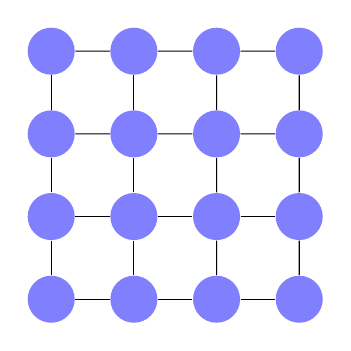
\begin{tikzpicture}[scale=0.7, darkstyle/.style={circle,fill=blue!50,minimum size=17}]
% nodes
  \foreach \x in {0,...,3}
    \foreach \y in {0,...,3} 
       {\pgfmathtruncatemacro{\label}{\x - 5 *  \y +21}
       \node [darkstyle]  (\x\y) at (1.5*\x,1.5*\y) {};} 

% connections
  \foreach \x in {0,...,3}
    \foreach \y [count=\yi] in {0,...,2}  
      \draw (\x\y)--(\x\yi) (\y\x)--(\yi\x) ;

\end{tikzpicture}

\end{center}
  \caption[Grid toy model]{$4 \times 4$ grid toy model used for an exact inference.}
    \label{fig:grid}
\end{figure}

Initially, the external field was set to $0$ and I considered the case when all couplings have the same value ranging from $-1$ to $1$. As it was expected, the naive mean field approach becomes an upper bound for the variational free energy. However, even in the case of this small model the TAP approximation for different values of couplings is either upper or lower bound. We can see that the approximation is closest to the ground truth when the couplings are close to zero. This is consistent with the fact that the approximation was performed around point where the temperature $T$ is infinite which means that spins are independent -- small values of couplings imitate this state.

Another computational inference problem that can be evaluate thanks to the TAP method is computing a mode of the marginal density for a given spin -- in this case we can estimate average value of the spin under the Boltzmann distribution. The right plot in the Figure \ref{fig:gridModel} shows the mean squared error (MSE) between the real and estimated magnetizations for all spins. In this case, the TAP approach provides much better estimates than the naive method -- we can see that adding a second term to the approximation allows to properly model the connections between the spins in the system. 

\begin{figure}[!htb]
\minipage{0.50\linewidth}%
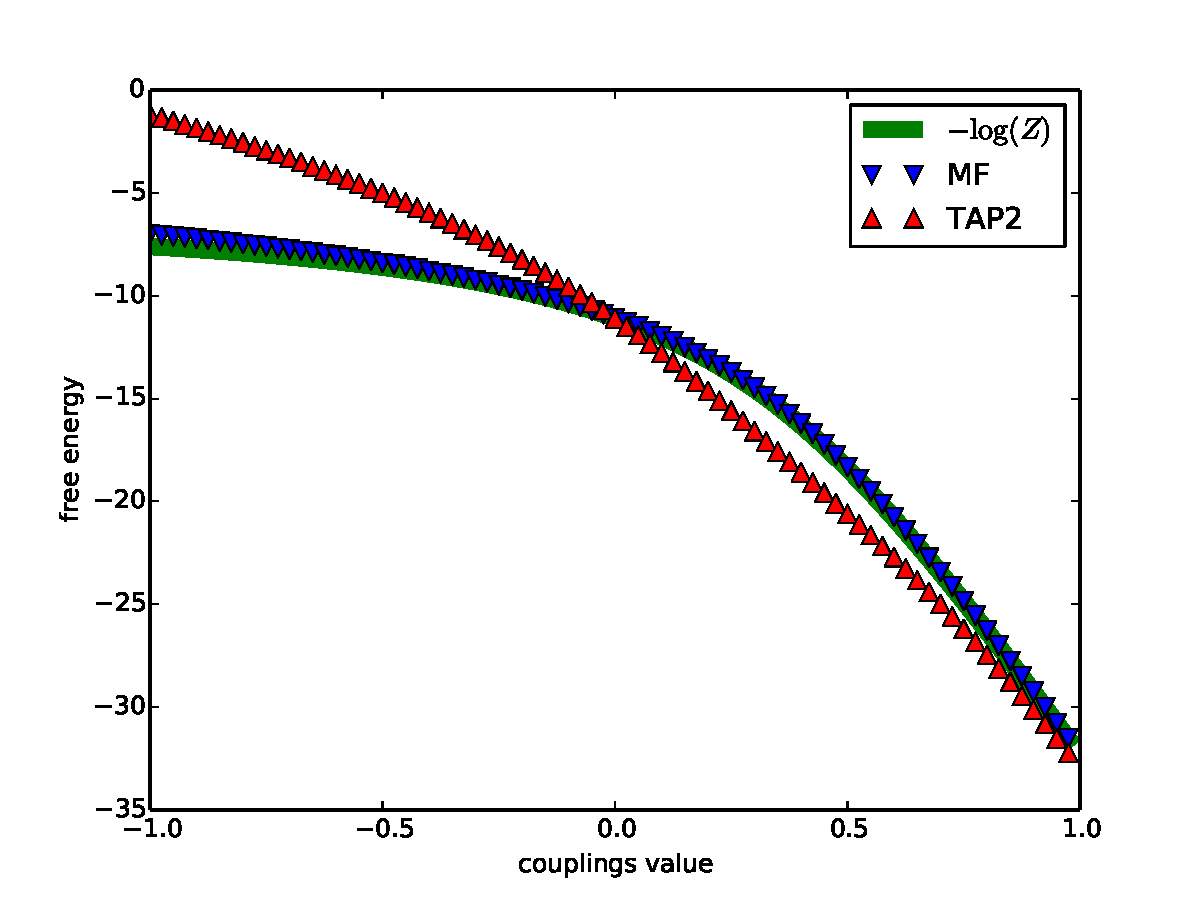
\includegraphics[width=\linewidth]{../../../Code/DRBM/toy/sameCouplingsZ}
\endminipage 
\minipage{0.50\linewidth}  
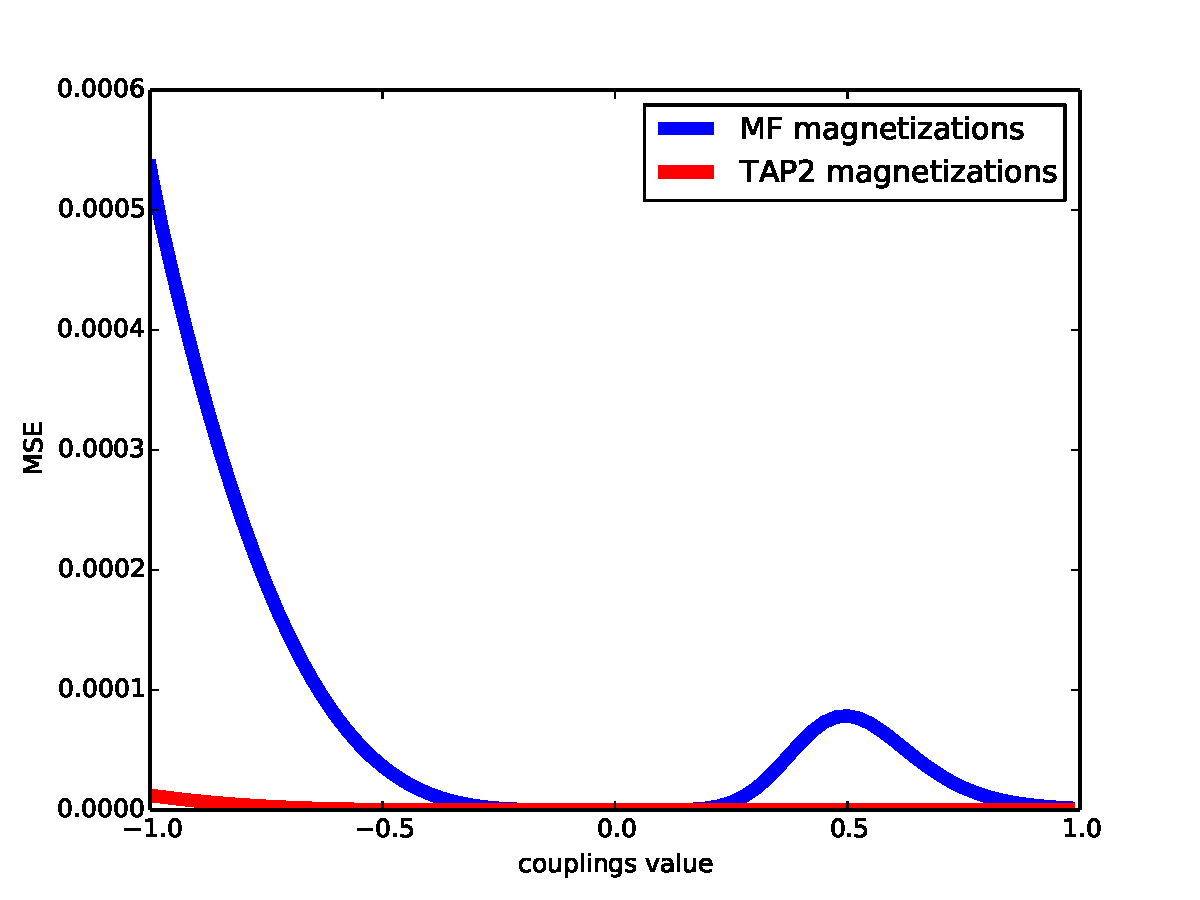
\includegraphics[width=\linewidth]{../../../Code/DRBM/toy/sameCouplingsMAG}
\endminipage\hfill
  \caption[Results on grid toy model with uniform couplings' strength]{Comparison of two  variational approaches -- free energy estimates (left) with the true free energy (green line) and MSE between real and estimated magnetisations (right) as a function of the couplings strength ranging from $-1$ to $1$.}
  \label{fig:gridModel}
\end{figure}

In the next experiment, all couplings were initialised to random values around "mean" strength which varies from $0$ to $1$ and then randomly assigned with positive or negative sign. The results are similar to the one observed previously (Figure \ref{fig:gridModelCoup}). The naive approach gives consistently better approximation for the $-\ln Z$ while the TAP method performs better in the case of estimating an average value of spin. 

\begin{figure}[!htb]
\minipage{0.50\linewidth}%
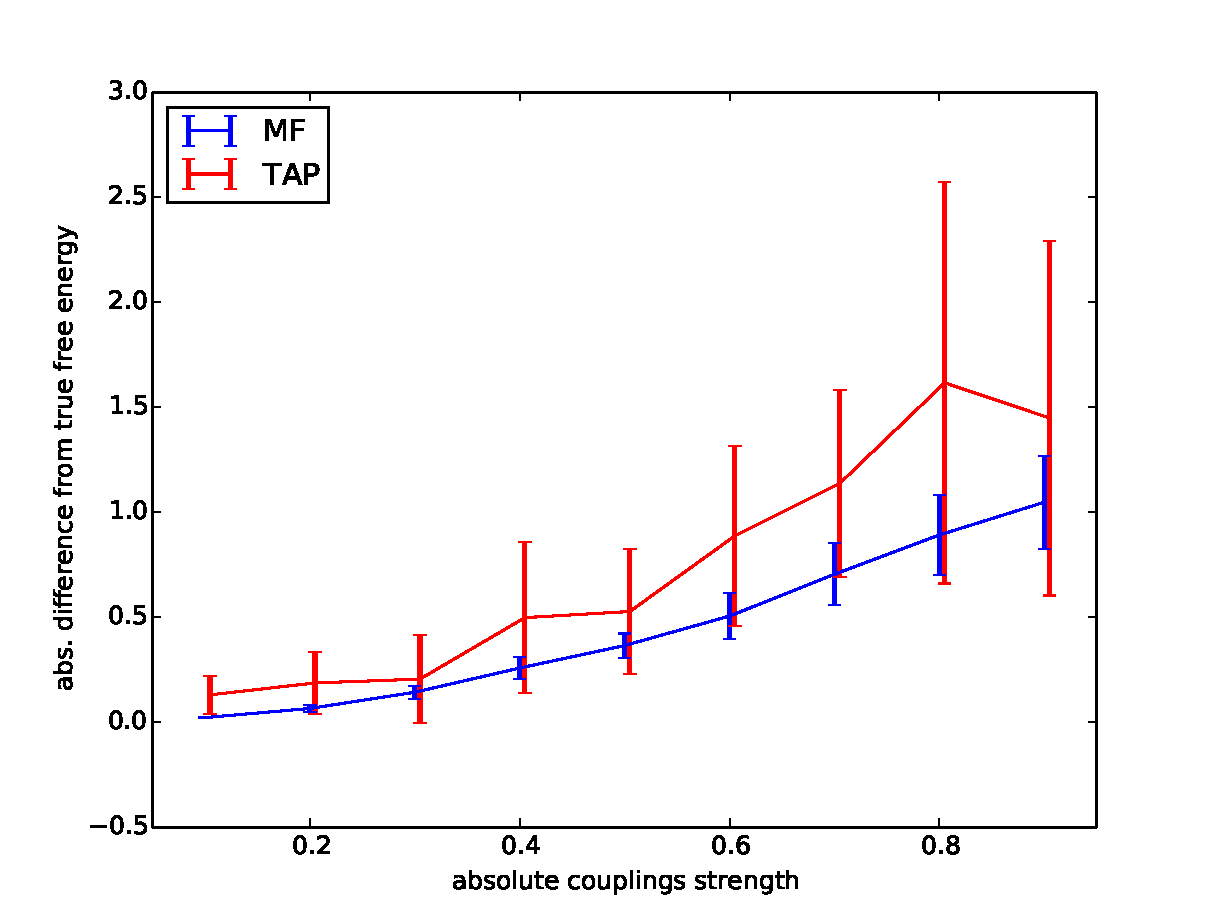
\includegraphics[width=\linewidth]{../../../Code/DRBM/toy/randomWeightsZ}
\endminipage 
\minipage{0.50\linewidth}  
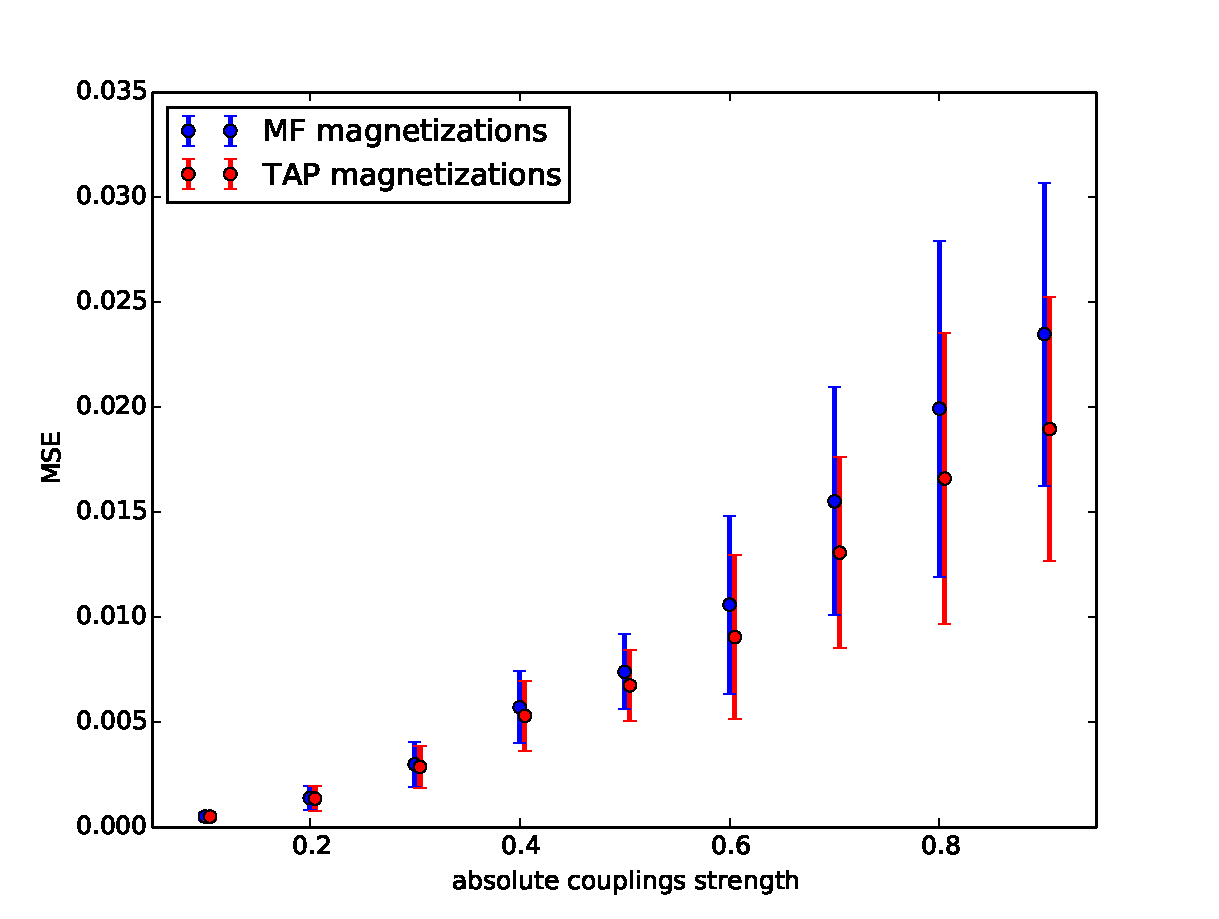
\includegraphics[width=\linewidth]{../../../Code/DRBM/toy/randomWeightsMAG}
\endminipage\hfill
  \caption[Results on grid toy model with random couplings' strength]{Absolute difference between true free energy and the one computed by the naive and the extended mean field approach (left) and MSE between real and estimated magnetisations (right) as a function of the absolute value of couplings strength.}
  \label{fig:gridModelCoup}
\end{figure}

The addition of external fields didn't change substantially the performance of methods  and the results are not included here.

\subsection{RBM toy model}
Due to the different structure of connections between states, the RBM toy model is less trivial to approximate. This should lead to considerably different results in the performance comparing to the toy mode  and it will be an another motivation to use the extended mean field approach on the real data set.

Unlike in the previous case, there is no strong heuristics how the updates of self-consistency relations should be performed. The literature suggests that in the case of the naive approach it is necessary to run self-consistency equations sequentially \cite{welling2002new}. To assess the impact on the final estimates, all three different schedules of updates will be considered here. Following the analysis from the previous section, initially all couplings were set to the same value ranging from $-1$ to $1$  (Figure 5).
\begin{figure}[!htb]
\minipage{0.50\linewidth}%
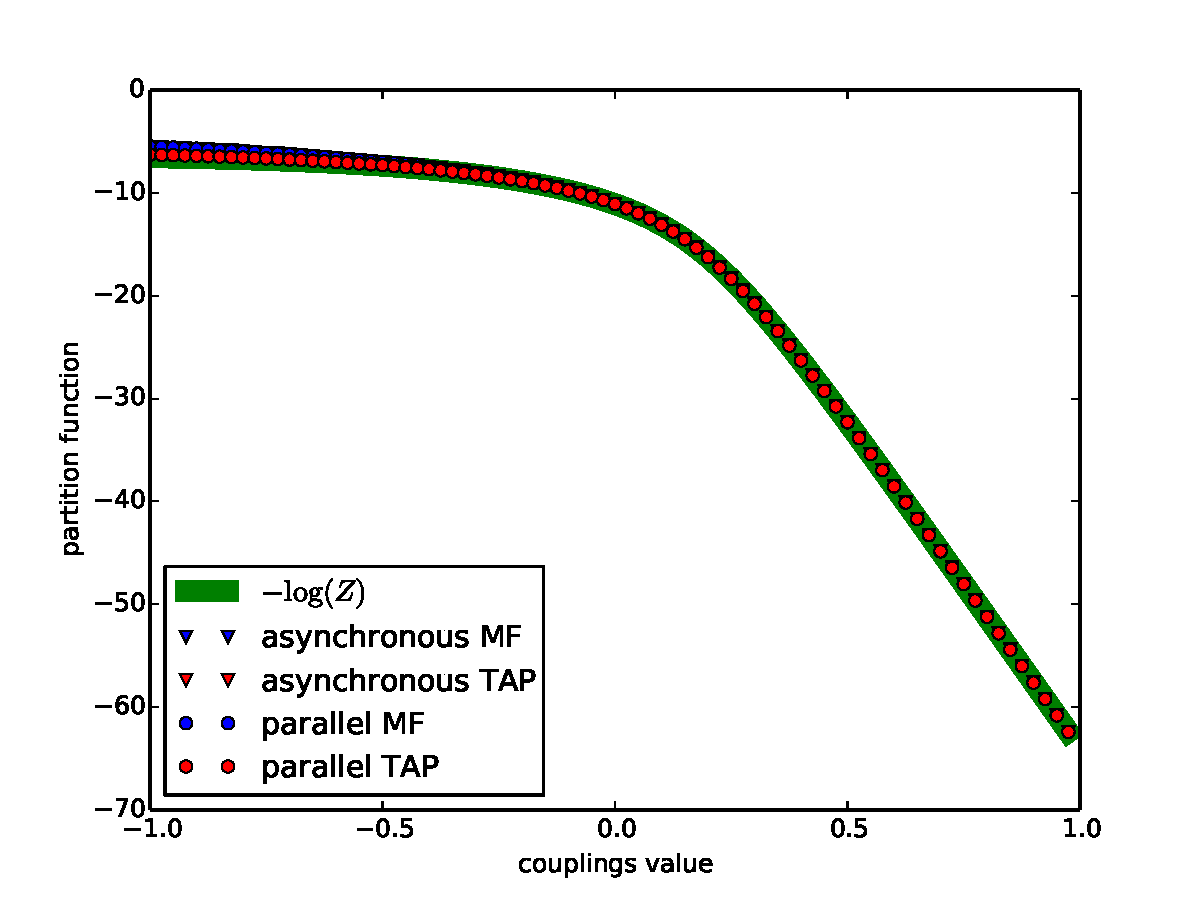
\includegraphics[width=\linewidth]{../../../Code/DRBM/toy/sameCouplingsRBMZ}
\endminipage 
\minipage{0.50\linewidth}  
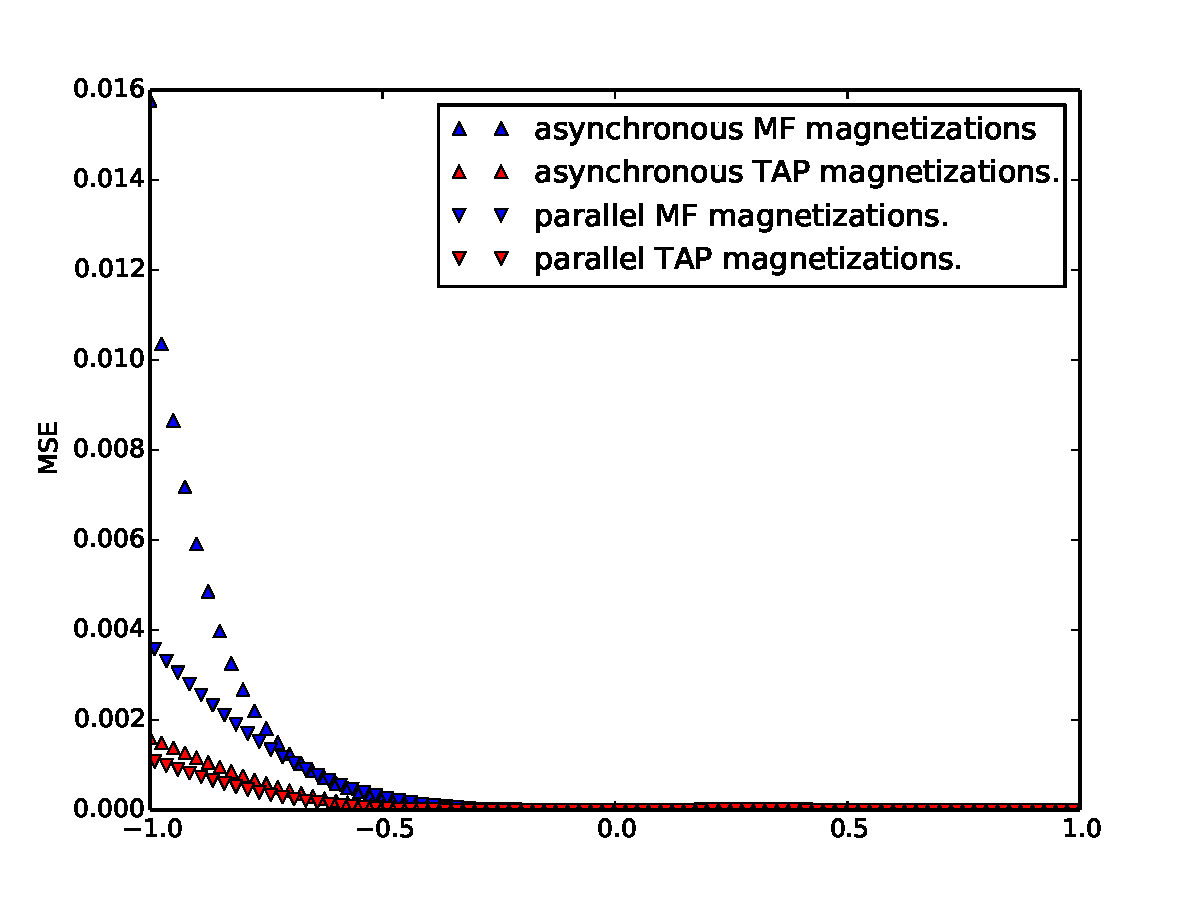
\includegraphics[width=\linewidth]{../../../Code/DRBM/toy/sameCouplingsRBMMAG}
\endminipage\hfill
\label{fig:rbmSame}
  \caption[Results on RBM toy model with uniform couplings' strength]{Comparison of two  variational approaches -- free energy estimates (left)with the true free energy (green line) and MSE between real and estimated magnetisations (right) as a function of the couplings strength ranging from $-1$ to $1$.}
\end{figure}

Unlike the case of the grid model, the estimation of the free energy is almost exact in the case of the TAP method while the naive mean field method again provides a slightly biased upper bound. As it was the case on the grid model, the magnetizations estimated using extended approximation are very precise while MF magnetizations shows discrepancies from true values when connections become stronger in the model. No significant differences were observed between different schedules of updates and thus results for sequential updates weren't included here.

When couplings were random with randomly assigned negative or positive signs, TAP approximation again yields consistently much better estimates that most of the time are exact at the same time having much smaller variance (Figure \ref{fig:rbmRandom}). Again, differences between schedules of updates were negligible and thus the results for sequential updates weren't included as they were almost identical to the ones obtained with asynchronous iterations.
\begin{figure}[!htb]
\minipage{0.50\linewidth}%
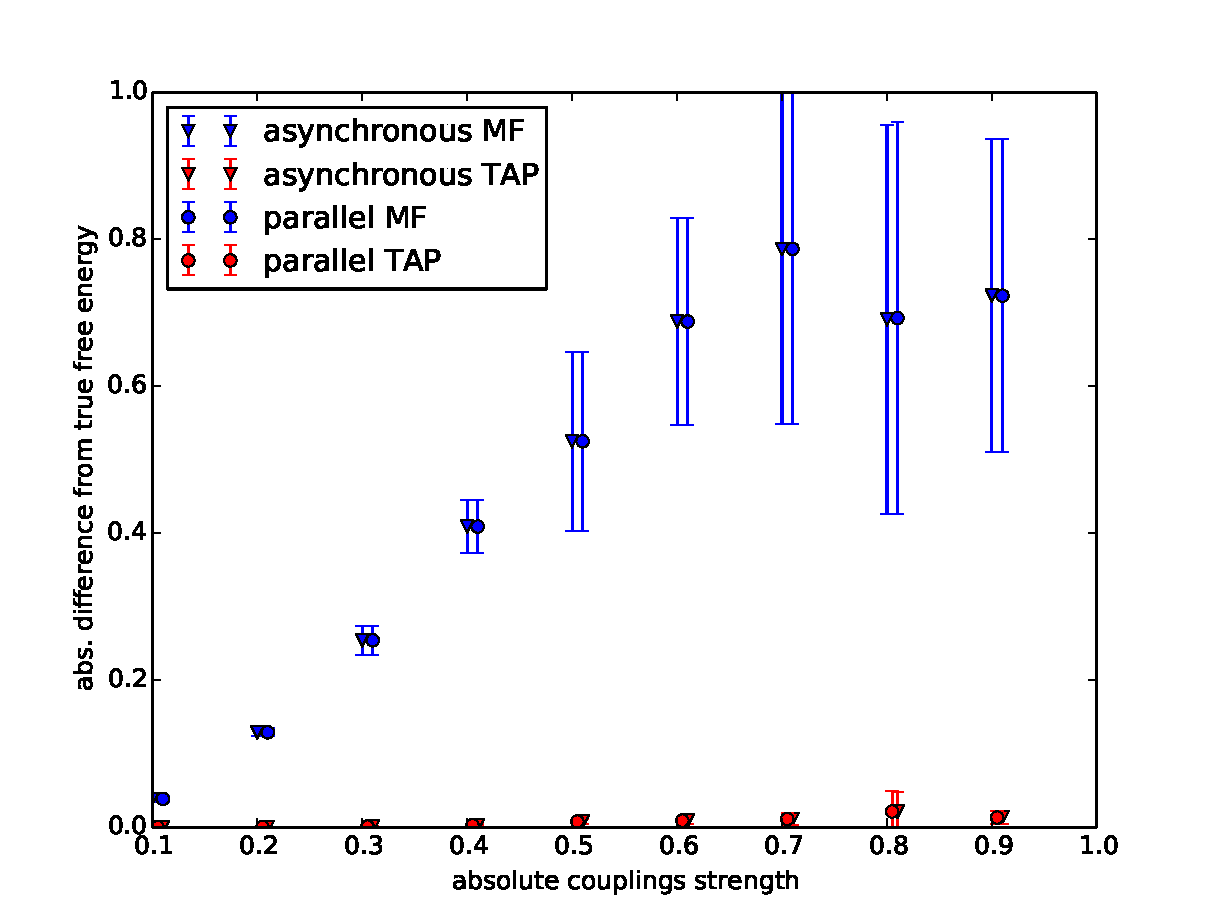
\includegraphics[width=\linewidth]{../../../Code/DRBM/toy/randomWeightsRBMZ}
\endminipage 
\minipage{0.50\linewidth}  
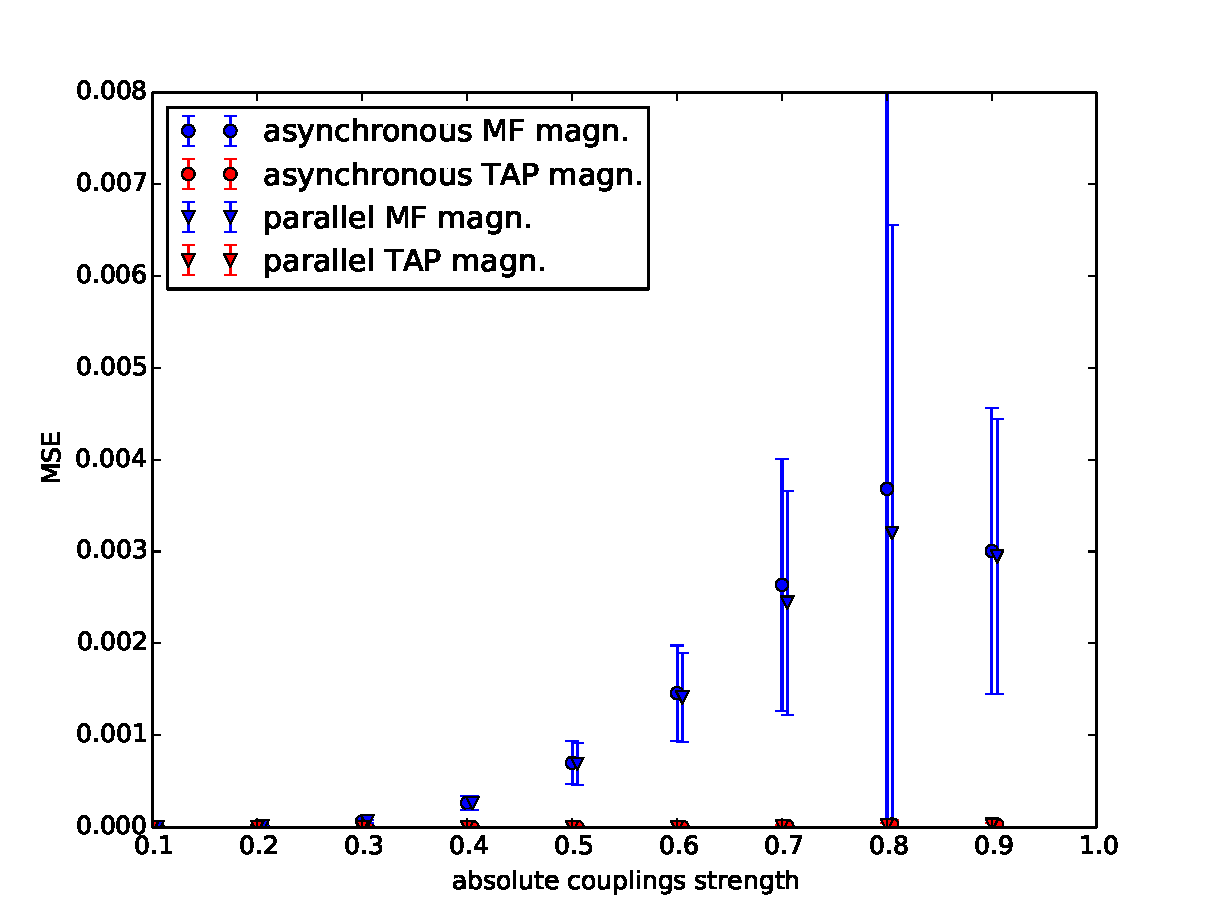
\includegraphics[width=\linewidth]{../../../Code/DRBM/toy/randomWeightsRBMMAG}
\endminipage\hfill
  \caption[Results on RBM toy model with random couplings' strength]{Absolute difference between the true free energy and the one computed by the naive and the extended mean field approach (left) and MSE between real and estimated magnetisations (right) as a function of the absolute value of couplings strength.}
  \label{fig:rbmRandom}
\end{figure}

The randomness associated with choosing the sign of connections might have averaged the overall statistics of the model, which in turn might affect the effectiveness of different schedules of updates. Thus, to assess how robust the analysed extended method is with different schedules, the couplings were chosen again randomly around given mean values but this time the sign of the weight was chosen sequentially (Figure \ref{fig:signs}).
\begin{figure}[!htb]
\minipage{0.50\linewidth}%
 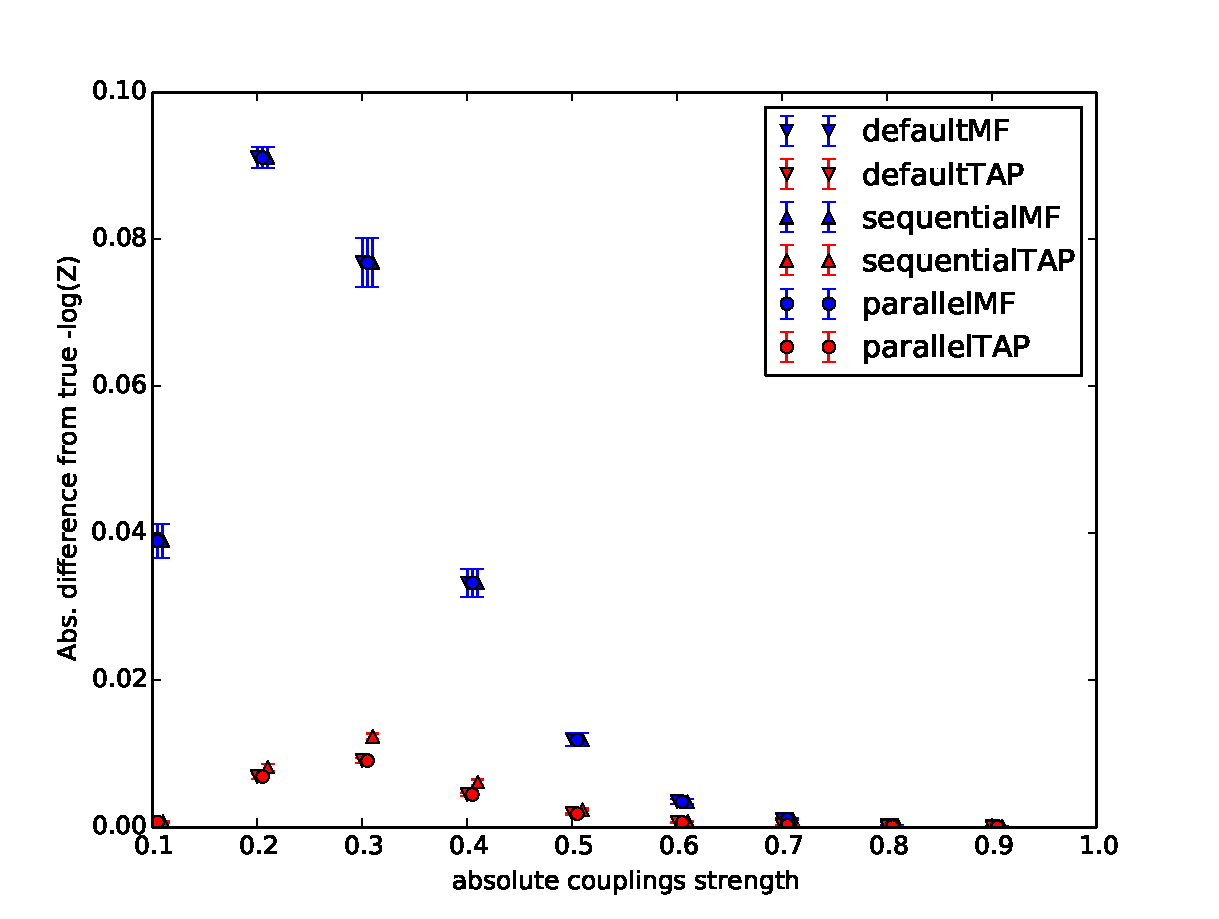
\includegraphics[width=\linewidth]{../../../Code/DRBM/toy/randomWeightsSignsRBMZ}
\endminipage 
\minipage{0.50\linewidth}  
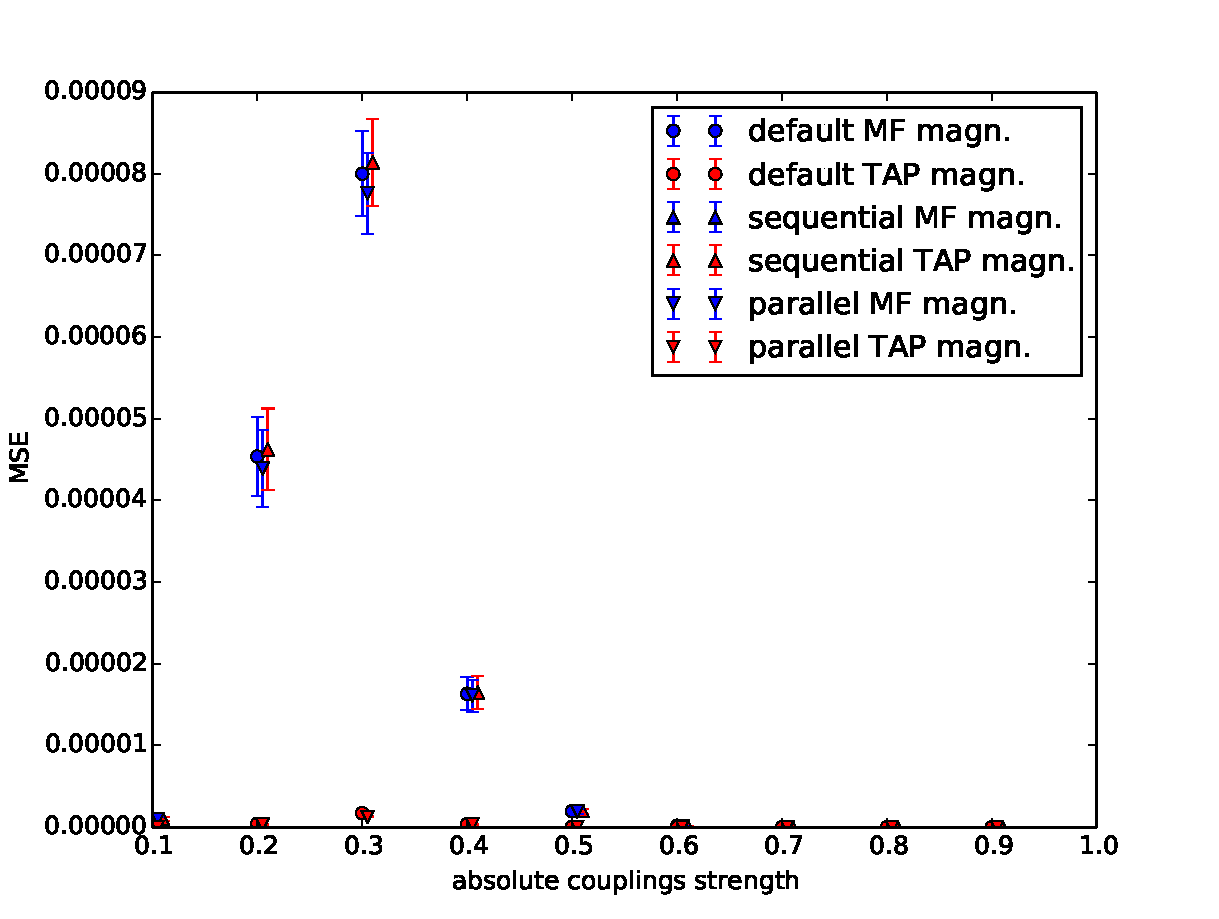
\includegraphics[width=\linewidth]{../../../Code/DRBM/toy/randomWeightsSignsRBMMAG}
\endminipage\hfill
  \caption[Results on RBM toy model with sequential changes of couplings' signs]{Absolute difference between the true free energy and the one computed by the naive and the extended mean field approach (left) and MSE between real and estimated magnetisations (right) as a function of the absolute value of couplings strength with sequentially opposite signs.}
  \label{fig:signs}
\end{figure}

This time, TAP estimates are not exact for couplings with an absolute strength around values $0.2$ or $0.3$. Moreover, the sequential updates yield very poor estimates for the magnetizations -- the MSE is almost the same as with the naive approach. The addition of external fields this time extensify the differences in performance between updates (Figure \ref{fig:bias}). The MSE between true and estimated magnetizations is higher for the TAP model with sequential updates than for the corresponding naive model.

\begin{figure}[!htb]
\minipage{0.50\linewidth}%
 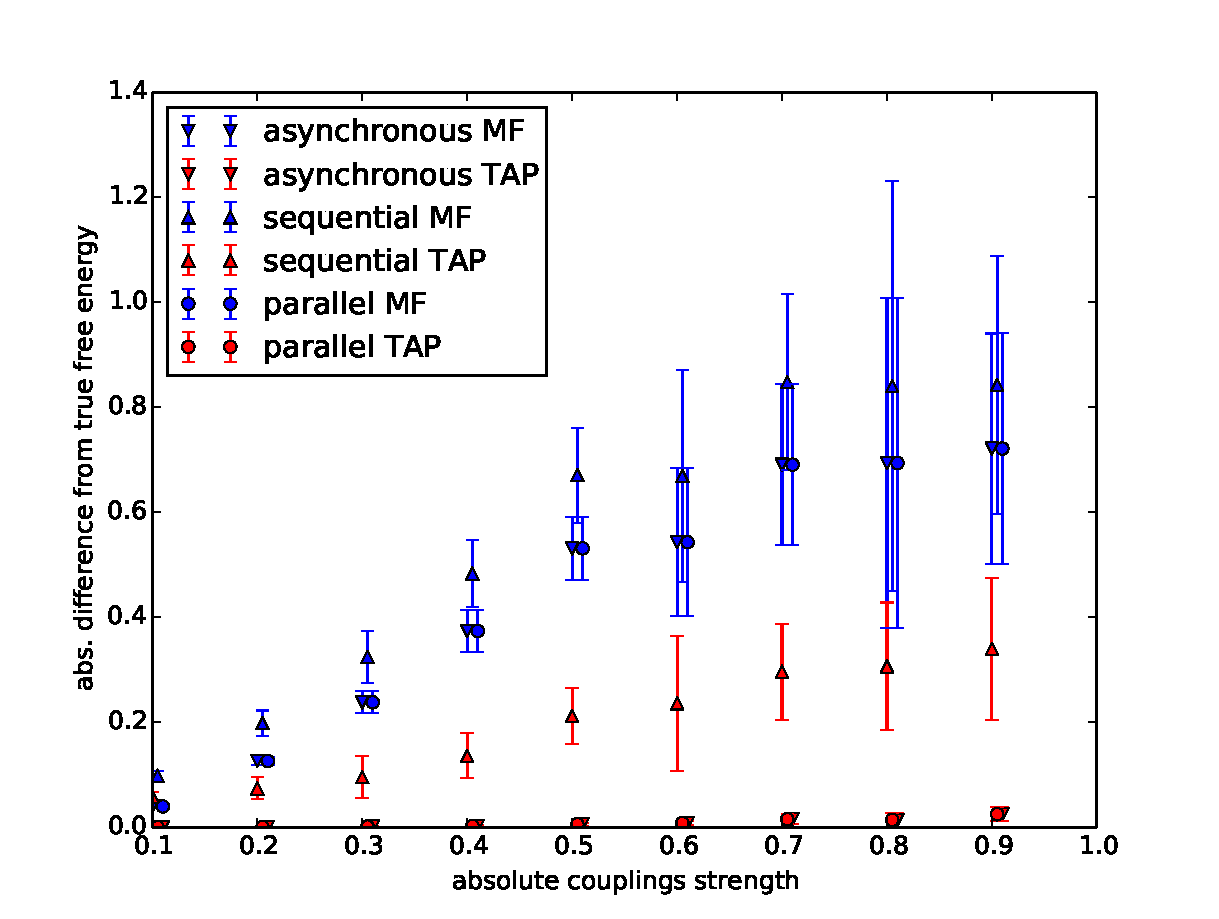
\includegraphics[width=\linewidth]{../../../Code/DRBM/toy/BrandomWeightsRBMZ}
\endminipage 
\minipage{0.50\linewidth}  
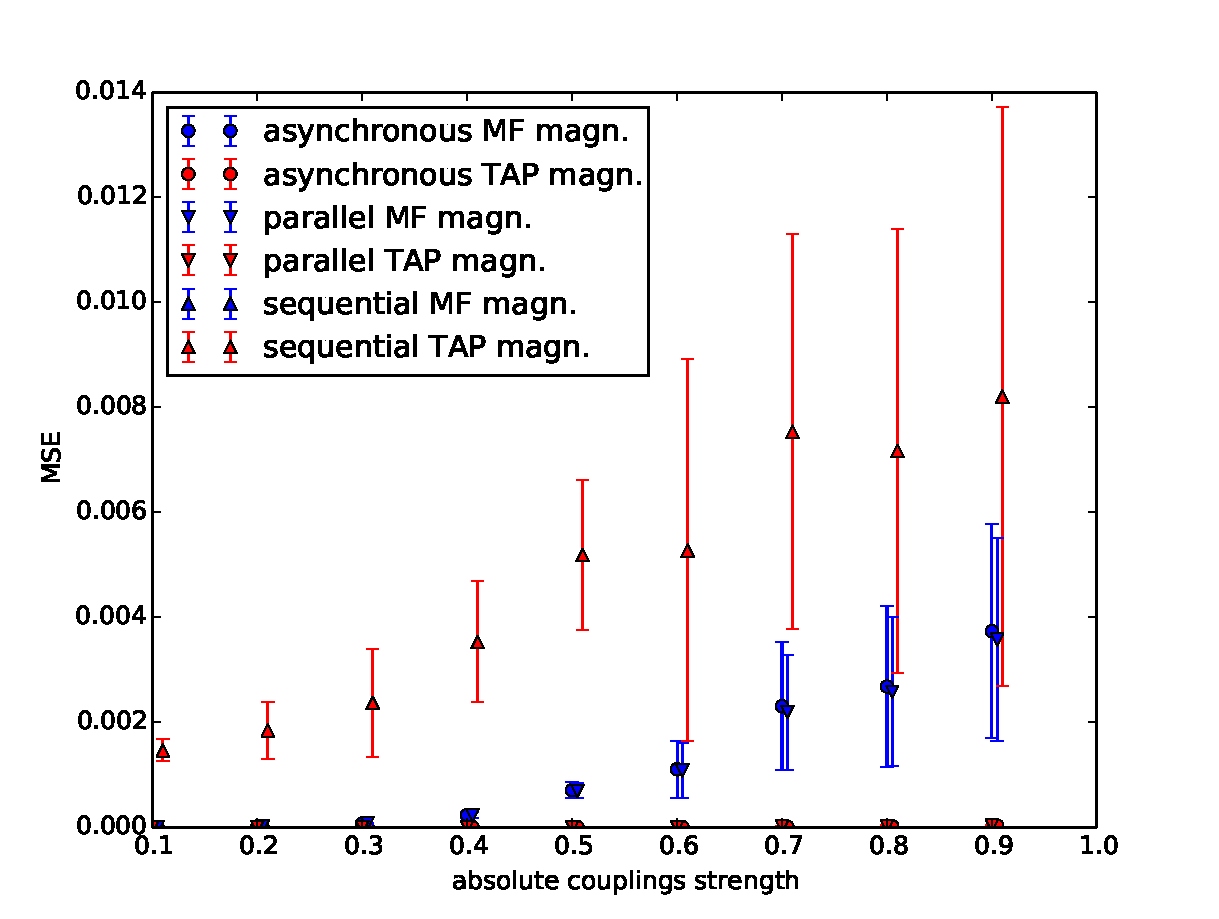
\includegraphics[width=\linewidth]{../../../Code/DRBM/toy/BrandomWeightsRBMMAG}
\endminipage\hfill
  \caption[Results on RBM toy model with external fields]{Absolute difference between true free energy and the one computed by naive and extended mean field approach (left) an MSE between real and estimated magnetisations (right) as a function of the absolute value of couplings strength with sequential changes of signs.}
  \label{fig:bias}
\end{figure}

Taking into consideration all results we can infer that the extended approximation yields robust results even though the expansion is performed at $\beta = 1$ and the couplings between the spins might have strong connections. Moreover, the real benefits of modelling the relationship between the spins can be observed when the MRF has the RBM structure. In this case the estimates of the free energy and the magnetizations were almost exact for the EMF-based model. However, contrary to the heuristics parallel updates perform just as well as the asynchronous ones while the sequential updates might drastically worsen the quality of estimates for the EMF-based models.


\chapter{Learning of Boltzmann machines}

\section{Unsupervised learning}
So far it was assumed that the couplings in analysed structures (along with bias terms) were known a priori. However, in general when we analyse some phenomena we don't know this values and we are interested in learning an unknown distribution $Q$ based on some observed data $\mathcal{D}$. The theoretical results suggests that the RBM structure is a natural candidate for approximating underlying distribution from which the data were generated. Thus, the unsupervised learning in this case consists of learning the parameters $\theta$ of the approximate distribution $P$. Therefore, our general goal is to maximize the probability of $\mathcal{D}$ under the MRF distribution i.e. we are looking for the vector of parameters $\mathbf{\theta}$ that maximize the likelihood given the training data:
\begin{align}
\begin{split}
\max_{\mathbf{\theta}} \ln \mathcal{L}(\mathbf{\theta}| \mathcal{D}) = \max_{\mathbf{\theta}}  \ln \prod_{i=1}^N p(\mathbf{v}_i |\mathbf{\theta}) = \max_{\mathbf{\theta}} \sum_{i=1}^N \ln p(\mathbf{v}_i |\mathbf{\theta} )
\end{split}
\end{align}
where $N$ is the size of $\mathcal{D}$. 

The experiments on toy models suggest that the initial unsatisfactory results with naive mean field approaches \cite{tieleman2008training} might be greatly improved if we include additional terms responsible for connections between the spins.

\subsection{Training of Boltzmann Machines}
With large graphical models, it is not possible to find an analytical solution to the maximum likelihood estimation of parameters and we need to resort to some approximation methods. That is also the case of the RBM and learning the parameters of this structure relies on the gradient ascent of the log-likelihood. At time $t$ during training, the update of the vector containing all parameters of the RBM $\mathbf{\theta}$ has the form:
\begin{align}
\begin{split}
\mathbf{\theta}^{t} = \mathbf{\theta}^{t-1} + \eta  \frac{\partial}{\partial \mathbf{\theta}^{t-1}}  \ln \mathcal{L}(\mathbf{\theta}| \mathcal{D}). 
\end{split}
\end{align}
This relies on the fact that the gradient w.r.t. parameters $\mathbf{\theta}$ informs us how fast function increases in the current point $\mathbf{\theta}^{t-1}$. 
By taking appropriately small learning rate, these iterative updates converge to stationary points. With large data set it is common to use a stochastic gradient ascent method \cite{robbins1951stochastic} where we sample a minibatch of datapoints and take a noisy gradient estimate which results in the update rule:
\begin{align}
\begin{split}
\mathbf{\theta}^{t+1} = \mathbf{\theta}^{t} + \eta \frac{1}{M} \frac{\partial}{\partial \mathbf{\theta}^t}  \sum_{m =1}^{M} \ln \mathcal{L}(\mathbf{\theta}| \mathbf{x}^{(m)}),
\end{split}
\label{eq:sgd}
\end{align}
where $M$ is the size of the minibatch. It can be shown that updates via \ref{eq:sgd} guarantee to converge to a local optimum under weak conditions \cite{bottou1998online}.

For a given data point $\mathbf{v}$ the log-likelihood can be seen as the difference between two energies:
\begin{align}
\begin{split}
\mathcal{L} = \ln P(\mathbf{v}) = -\ln (\sum_{\mathbf{h}} e^{-E(\mathbf{v,h})} ) -\ln Z = F^c(\mathbf{v}) + F
\end{split}
\label{eq:loglikelihood}
\end{align}
where $F$ is the \emph{free energy} of the RBM and $F^c$ denotes the clamped free energy as we operate on the fixed visible units $\mathbf{v}$. The gradient of the log-likelihood w.r.t $\theta$ given a training example $\mathbf{v}$ takes the form:
\begin{align}
\begin{split}
\frac{\partial \log \mathcal{L}(\mathbf{\theta  | \mathbf{v}})}{\partial \mathbf{\theta}} & = \frac{\partial F^c }{\partial \mathbf{\theta}} - \frac{\partial F }{\partial \mathbf{\theta}} \\
& = - \frac{\sum_{\mathbf{h}} e^{-E(\mathbf{v,h})} \frac{\partial E(\mathbf{v,h})}{\partial \mathbf{\theta}}}{\sum_{\mathbf{h}} e^{-E(\mathbf{v,h})}} + \frac{\sum_{\mathbf{v, h}} e^{-E(\mathbf{v,h})} \frac{\partial E(\mathbf{v,h})}{\partial \mathbf{\theta}}}{\sum_{\mathbf{v, h}} e^{-E(\mathbf{v,h})}} \\
& = - \sum_\mathbf{h} p(\mathbf{h} | \mathbf{v}) \frac{\partial E(\mathbf{v,h})}{\partial \mathbf{\theta}} +  \sum_\mathbf{v, h} p(\mathbf{v}, \mathbf{h}) \frac{\partial E(\mathbf{v,h})}{\partial \mathbf{\theta}} \\
& =  - \mathbb{E}_{p(\mathbf{h} | \mathbf{v})} \left( \frac{\partial E(\mathbf{v,h})}{\partial \mathbf{\theta}} \right) + \mathbb{E}_{ p(\mathbf{v,h}) } \left( \frac{\partial E(\mathbf{v,h})}{\partial \mathbf{\theta}} \right)
\label{eq:gradient}
\end{split}
\end{align}

As we can see the gradient is the difference of two expectations -- the expected value of the gradient of the energy function under the model distribution and under the conditional distribution of the hidden variables given the observed variables $\mathbf{v}$. Thanks to the restriction imposed on the structure of the Boltzmann machine, the clamped free energy can be computed explicitly. However, as it was mentioned previously, direct calculations of the second term leads to the complexity that is exponential in the number of variables in the model.

\subsection{Monte Carlo methods}
The second expectation from the gradient in \ref{eq:gradient} is intractable to compute explicitly  in the case of large models and we have to resort to some kind of approximations. Monte Carlo methods rely on stochastic generations of random variables w.r.t. the desired expectation needs to be computed. Denote by:
$$ \theta = \mathbb{E}_p(f(X)) = \int f(\mathbf{x})p(\mathbf{x}) \text{d}\mathbf{x}$$
the quantity of interest where $X \sim p(\cdot)$. The Monte Carlo estimate has the form:
$$ \hat{\theta} = \frac{1}{N} \sum_{i=1}^N f(\mathbf{x}^i)$$
where $\mathbf{x}^i$, $i \in \{1,..., N\}$ are random samples from $X$ and $N$ is the number of samples. This simple procedure provides unbiased and consistent estimate of $\theta$ as $n \rightarrow \infty$.

\subsubsection{Markov chain Monte Carlo}
Monte Carlo method relies on the fact that we are able to generate independent random samples from the distribution of interest. In the case of the RBM, we are not able to generate random samples $\{ \mathbf{v,h} \}$ from the complex joint posterior to approximate the expectation of interest. However, we can use Monte Carlo Markov chain (MCMC) framework to generate approximate samples from the joint distribution $p( \mathbf{v,h} )$.

A discrete stochastic process $X = \{ X_t, t \in \mathbb{N} \}$ which takes values in discrete set $S$ is a Markov chain if the Markov property holds, i.e.
$$p_{ij}^t = P(X_t = j | X_{t-1} = i,  ..., X_{0} = i_0) = P(X_t = j | X_{t-1} = i)$$
for every $t \in \mathbb{N}$ and $i,j, i_0 \in S$. In the case of the discrete process, we usually operate on the transition matrix defined as $\mathbf{P} = (p_{ij})_{i,j \in S}$. The fundamental concept of the theory of the MCMC is stationarity or a stationary distribution $\mathbf{\pi}$ for which it holds $\mathbf{\pi} = \mathbf{P\pi}.$ MCMC methods focus on constructing an appropriate Markov chain that converges to the desired distribution.

\subsubsection{Gibbs sampling}
A particular class of MCMC algorithms is the Gibbs sampling algorithm which enables us to produce samples from the joint probability distribution using full conditional distributions. This method is also often called "block-at-a-time" as the transition probabilities are related with subblocks of the vector $\mathbf{x}$. Let $\mathbf{x}$ be divided into two blocks of variables $\mathbf{x}_1$ and $\mathbf{x}_2$. The Gibbs sampler subsequently generates samples from $\mathbf{x}_1^i = p(\mathbf{x}_1 | \mathbf{x}_2)$ and $\mathbf{x}_2^i = p(\mathbf{x}_2 | \mathbf{x}_1)$ which forms samples from the joint $(\mathbf{x}_1^i, \mathbf{x}_2^i)$ assuming we reached a convergence of the chain.
     
In the case of the RBM, the structure of the model suggests that we can divide the variables from the joint into two blocks -- visible and hidden units. No connections between variables from the same layer enables us efficiently sample from conditionals $p(\mathbf{v}| \mathbf{h})$ and $p(\mathbf{h} | \mathbf{v})$ using \ref{gibbs}.
    
\subsection{Contrastive Divergence}
The main challenge related with MCMC methods is the computational burden related with ensuring that the Markov chain has been run sufficiently long to ensure convergence to a stationary distribution. However, it was proven empirically that the chain might be run only a few steps in order to train an effective model \cite{hinton2002training} which is called contrastive divergence (CD) learning. 
 
There are two steps which differ CD from the naive MCMC sampling to approximating the second expectation from the gradient \ref{eq:gradient}. Firstly, instead of running the Markov chain until it obtains a stationary distribution, the chain is initialized using training data point $\mathbf{v}^{0}$ from the training data set. Secondly, the Gibbs chain is run only for $k$ steps (CD-$k$) where $k$ is usually smaller than $20$. 
Figure \ref{fig:gibbsSampling} presents the procedure for the CD-$1$:
 \begin{figure}[!htb]
\begin{center}
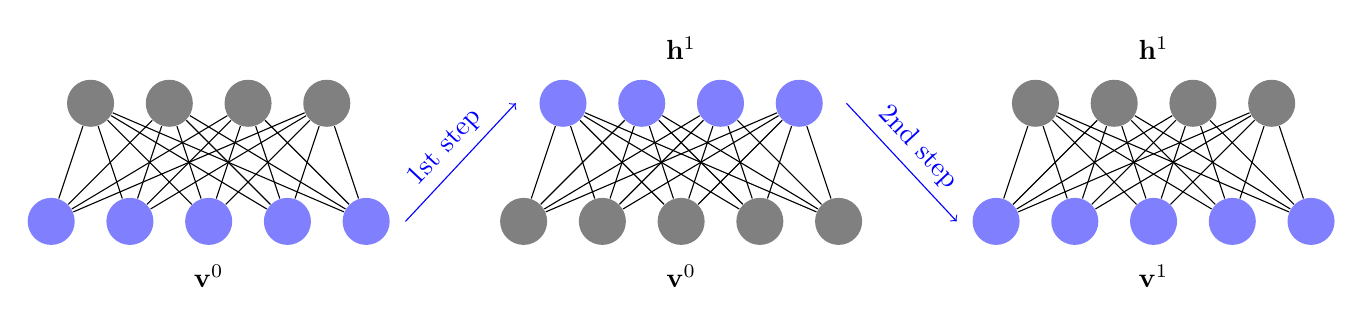
\begin{tikzpicture}[darkstyle/.style={circle,fill=black!50,minimum size=20}]
    \tikzstyle{every pin edge}=[<-,shorten <=1pt]
    \tikzstyle{neuron}=[circle,fill=black!25,minimum size=17pt,inner sep=0pt]
    \tikzstyle{input neuron}=[neuron, fill=blue!50];
    \tikzstyle{hidden neuron}=[neuron, fill=black!50];
     \tikzstyle{shidden neuron}=[neuron, fill=blue!50];
          \tikzstyle{thidden neuron}=[neuron, fill=black!50];
    \tikzstyle{annot} = [text width=4em, text centered]

    % Draw the input layer nodes
    \foreach \name / \y in {1,...,5}
    % This is the same as writing \foreach \name / \y in {1/1,2/2,3/3,4/4}       
     \node[input neuron] (I-\name) at (-\y, 0) {};

    % Draw the hidden layer nodes
\foreach \name / \y in {1,...,4}
	\node[hidden neuron] (H-\name) at (-\y -.5, 1.5) {};

    \foreach \source in {1,...,5}
        \foreach \dest in {1,...,4}
            \path (I-\source) edge (H-\dest);
            
            
    % Draw the input layer nodes
    \foreach \name / \y in {1,...,5}
    % This is the same as writing \foreach \name / \y in {1/1,2/2,3/3,4/4}       
     \node[hidden neuron] (II-\name) at (-\y +6, 0) {};

    % Draw the hidden layer nodes
\foreach \name / \y in {1,...,4}
	\node[input neuron] (HH-\name) at (-\y -.5 +6, 1.5) {};

    \foreach \source in {1,...,5}
        \foreach \dest in {1,...,4}
            \path (II-\source) edge (HH-\dest);
            
% Draw the input layer nodes
    \foreach \name / \y in {1,...,5}
    % This is the same as writing \foreach \name / \y in {1/1,2/2,3/3,4/4}       
     \node[input neuron] (III-\name) at (-\y +12, 0) {};

    % Draw the hidden layer nodes
\foreach \name / \y in {1,...,4}
	\node[hidden neuron] (HHH-\name) at (-\y -.5 +12, 1.5) {};

    \foreach \source in {1,...,5}
        \foreach \dest in {1,...,4}
            \path (III-\source) edge (HHH-\dest);
            
            \draw[->, blue] (-.5,0) -- node[above,sloped] {1st step} (.9,1.5);
                \draw[->, blue] (-.9 + 6,1.5)-- node[above,sloped] {2nd step} (.5 + 6,0);
             
            \draw    (-3,-.7) node {$\mathbf{v}^{0}$};
          %  \draw    (-3,2.2) node {$\mathbf{h}^{0}$};
            \draw    (-3 + 6,-.7) node {$\mathbf{v}^{0}$};
            \draw    (-3 +6,2.2) node {$\mathbf{h}^{1}$};
            \draw    (-3+ 12,-.7) node {$\mathbf{v}^{1}$};
            \draw    (-3 +12,2.2) node {$\mathbf{h}^{1}$};
\end{tikzpicture}
\end{center}
  \caption[1]{The first step of the Gibbs sampler for the RBM for a particular data point $\mathbf{v}^0 \in \mathcal{D}$.}
  \label{fig:gibbsSampling}
\end{figure}

The approximation to the gradient by the single data point $\mathbf{v}^0$ in the case of CD-$k$ takes the form:
\begin{align}
\begin{split}
- \sum_\mathbf{h} p(\mathbf{h} | \mathbf{v}^0) \frac{\partial E(\mathbf{v}^0, \mathbf{h})}{\partial \mathbf{\theta}} +  \sum_{\mathbf{h}} p(\mathbf{h} | \mathbf{v}^k) \frac{\partial E(\mathbf{v}^k,\mathbf{h})}{\partial \mathbf{\theta}} 
\label{eq:gradientCD}
\end{split}
\end{align}
It should be noted here that as we run the Gibbs chain only a few ($k$) steps, the samples $\{\mathbf{v}^k, \mathbf{h}^k\}$ don't come from the stationary distribution and the approximation \ref{eq:gradientCD} is biased as it doesn't maximize the likelihood of the data but the difference of two KL-divergences \cite{hinton2002training}, \cite{fischer2012introduction}:
$$KL(Q | P) - KL (P_k| P)$$
where $Q$ is the empirical distribution and $P_k$ is the distribution after $k$ step of the Gibbs chain and this explains the name of the algorithm.
\subsubsection{Persistent contrastive divergence}  
It was observed that the contrastive divergence procedure still requires many steps to be run in order to learn a good generative model. The rate of learning might be significantly improved when we don't reinitialize the Markov chains with a new training batch in order to obtain a sample $\{\mathbf{v}_i^k\}_{i=1}^N$ where $N$ is the size of the batch but rather keep "persistent" chains (PCD) \cite{tieleman2008training}. Thus, the starting state for the Gibbs chain is equal to the last step from the previous update. The assumption made here is that between parameter updates, the model changes only slightly in terms of parameters' values\cite{neal1992connectionist}. Thus, the initialization from the last state of the Gibbs chain taken from the previous model should be closer to the model distribution. The empirical results suggest to keep one persistent chain per one training data point in a batch.

\subsection{Learning using extended mean field approximation}
The stochastic procedure described in the previous section can be exchanged with the fully deterministic approach as the log-likelihood in the case of the EMF approximation has the form:
\begin{align}
\begin{split}
\mathcal{L} = \ln P(\mathbf{v}) = F^c(\mathbf{v}) - F^{EMF}.
\end{split}
\label{eq:emfLL}
\end{align}
As the first term from \ref{eq:loglikelihood} can be computed explicitly, it is independent from the approach taken during training and we only have to derive the updates using the EMF approximation of the free energy.

Let's now fix visible and hidden magnetizations $\{ \mathbf{m}^v, \mathbf{m}^h \}$. The gradient of the log-likelihood w.r.t a coupling parameter $W_{ij}$ up to the third-order term is:
\begin{align*}
\begin{split}
\frac{\partial F^{EMF}}{\partial W_{ij}} = & -m_i^v m_j^h - W_{ij}^t(m_i^v - (m_i^v)^2)(m_j^h - (m_j^h)^2) \\
 & - 2W_{ij}^2 (m_i^v - (m_i^v)^2)(\frac{1}{2} - m_i^v)(m_j^h - (m_j^h)^2)(\frac{1}{2} - m_j^h),
\end{split}
\end{align*}
while the updates for the bias terms are just negative of the fixed-point magnetizations:
\begin{align}
\begin{split}\frac{\partial F^{EMF}}{\partial a_i} &= -m_i^v, \\
\frac{\partial F^{EMF}}{\partial b_j} & = -m_j^h.
\end{split}
\end{align}
Thus, the training procedure using a deterministic approach goes as follows: given a data point $\mathbf{v}$ we obtain expected values of the hidden units $\mathbf{h} = \text{sigm} ( W\mathbf{v} + \mathbf{b})$ which are starting points for magnetizations, i.e. $\mathbf{m}^v_0 = \mathbf{v}$ and $\mathbf{m}^{h}_0 = \mathbf{h}$. Then, we perform an iterative algorithm (which can have the form as presented in the previous chapter) until convergence to obtain magnetizations $\{ \mathbf{m}^v,\mathbf{m}^h\}$ that satisfy self-consistency relations. Those magnetizations can then be used to obtain gradient w.r.t the parameters of the model and to compute the approximation of the free energy.
 
\subsection{Approximating the log-likelihood}
The problems related with intractability of the partition function makes training such structure very difficult as we cannot observe directly progress of learning. Thus, we need to resort to some approximations. One of the most popular approaches to measure progress in training RBMs is due to Besag \cite{besag1972nearest} -- consider the following approximation of $n$-dimensional distribution
\begin{equation}
P(\mathbf{x}; \theta) = \prod_i p(x_i| x_1,...,x_{i-1};\theta) \approx \prod_i p(x_i | x_1, ..., x_{i-1}, x_{i+1},..., x_n;\theta) = \prod_i p(x_i| x_{-i} ;\theta) \coloneqq PL (\mathbf{x};\theta) 
\end{equation}
where the first equation comes from the chain rule and $x_{-i}$ denotes the set of all variables except variable $x_i$. We assume here that marginals given all other are independent of each other. The likelihood has then the form:
\begin{equation}
\ln PL(\mathbf{x}; \theta) = \sum_i \ln P(x_i | x_{i-1} ;\theta).
\end{equation}
If the analysed phenomena has many dimensions this approximation is still computationally expensive. Thus, another step is to choose only one marginal as a proxy, i.e.
\begin{equation}
\ln PL(\mathbf{x}; \theta) = n \ln P(x_i | \mathbf{x}_{-i} ; \theta),
\end{equation}
where $i$ is randomly chosen from $\{1,2, ..., n\}$. It can be shown that this pseudo-likelihood is maximized by the true parameters of the model. In the case of the RBM, this estimator takes especially efficient form:
\begin{align}
\begin{split}
\ln PL(\mathbf{x}; \theta) \approx n \log \left( \frac{\exp\{- F^c(\mathbf{x})\}}{\exp\{-F^c(\mathbf{\hat{x}})\} + \exp\{- F^c(\mathbf{x})\}} \right) = n \ln \left( \text{sigm}(F^c(\mathbf{\hat{x}}) - F^c(\mathbf{x}) \right)
\label{eq:pseudoLL}
\end{split}
\end{align}
where $\mathbf{\hat{x}}$ represents the vector $\mathbf{x}$ with $i$-th variable flipped, i.e. $1-x_i$.

\subsection{Real scale model -- MNIST data set}
The data set that will be used for the comparison and the evaluation of EMF and CD training algorithms is the MNIST set \cite{lecun1998} which is a well-known benchmark image classification dataset that consists of $60000$ training and $10000$ testing images of digit numbers. They are represented
on $28$-by-$28$ grey-scale grid of pixels. Thus, the first visible layers in all analysed models consists of $784$ visible units. Following \cite{gabrie2015training}, \cite{salakhutdinov2008learning} all images were rescaled to $ \lbrace 0, 1 \rbrace $ and binarized by setting all non-zero pixels to $1$ in all experiments.
The data set was divided into $600$ mini-batches which results in $100$ training points per batch.

\subsection{Comparison of both approaches}
In order to test the efficiency of the EMF learning algorithm, I used three expansions of $\ref{eq:varFreeEnergy}$ -- up to the first-order (MF), second-order (TAP2) and third order (TAP3) term. Moreover, I varied the number of iterations of self-consistency relations ($3$ and $10$) using asynchronous updates of the form \ref{eq:asynch} to mimic the idea from the contrastive divergence approach. As a benchmark, two models were trained following the stochastic training (CD$1$, CD$10$).

Furthermore, all models described above were trained using persistent approach (PMF, PTAP2, PTAP3, PCD). In the case of the EMF approximation, the magnetizations of a batch  from the previous update are the starting points in the next update \cite{gabrie2015training}. Similarly to PCD, this idea is based on the fact that between updates the model changes only slightly and it should improve the convergence to the new fixed point magnetizations.

All models were trained $10$ times using the same set-up of free parameters with $500$ units. The purpose of this experiment is to compare different RBM trainings thus following \cite{gabrie2015training} I didn't use the adaptive learning rate which was set to $0.005$, learning was performed using mini-batch updates with $100$ training points per batch. The couplings matrix was randomly initialised using normal distribution with zero mean and variance set to $0.01$. This allows to compare the procedures in the their "raw" forms. 

However, the EMF approximation was performed around the infinite temperature were the spins are independent. Thus, in general couplings should have small values -- this can be enforced using regularization which at the same times allows for a better generalization. From probabilistic perspective this can be seen as adding a weighted prior over the parameters (maximum a posteriori training). The criterion that will be maximized has now the form:
\begin{align}
\begin{split}
E(\theta, \mathcal{D}) = \ln \mathcal{L}(\mathbf{\theta}| \mathcal{D}) - \lambda R(\theta)
\end{split}
\end{align}
where $R(\cdot)$ is the regularizer and $\lambda \in \mathbb{R}_+$ is a hyper-parameter which controls the effective power of the regularization.
In all experiments Laplacian prior $R(\theta) = \| \theta \|_1$ ($L1$ regularization) was used with $\lambda$ set to $0.01$. 

Figure \ref{fig:validLL} presents the pseudo log-likelihood \ref{eq:pseudoLL} (left) and EMF log-likelihood \ref{eq:emfLL} for the non-persistent training procedure. Firstly, by the visual inspection both approximation yield very similar results for each analysed model. However, the EMF estimates are much less noisy at a lower computational cost.

\begin{figure}[!htb]
\minipage{0.50\linewidth}%
%  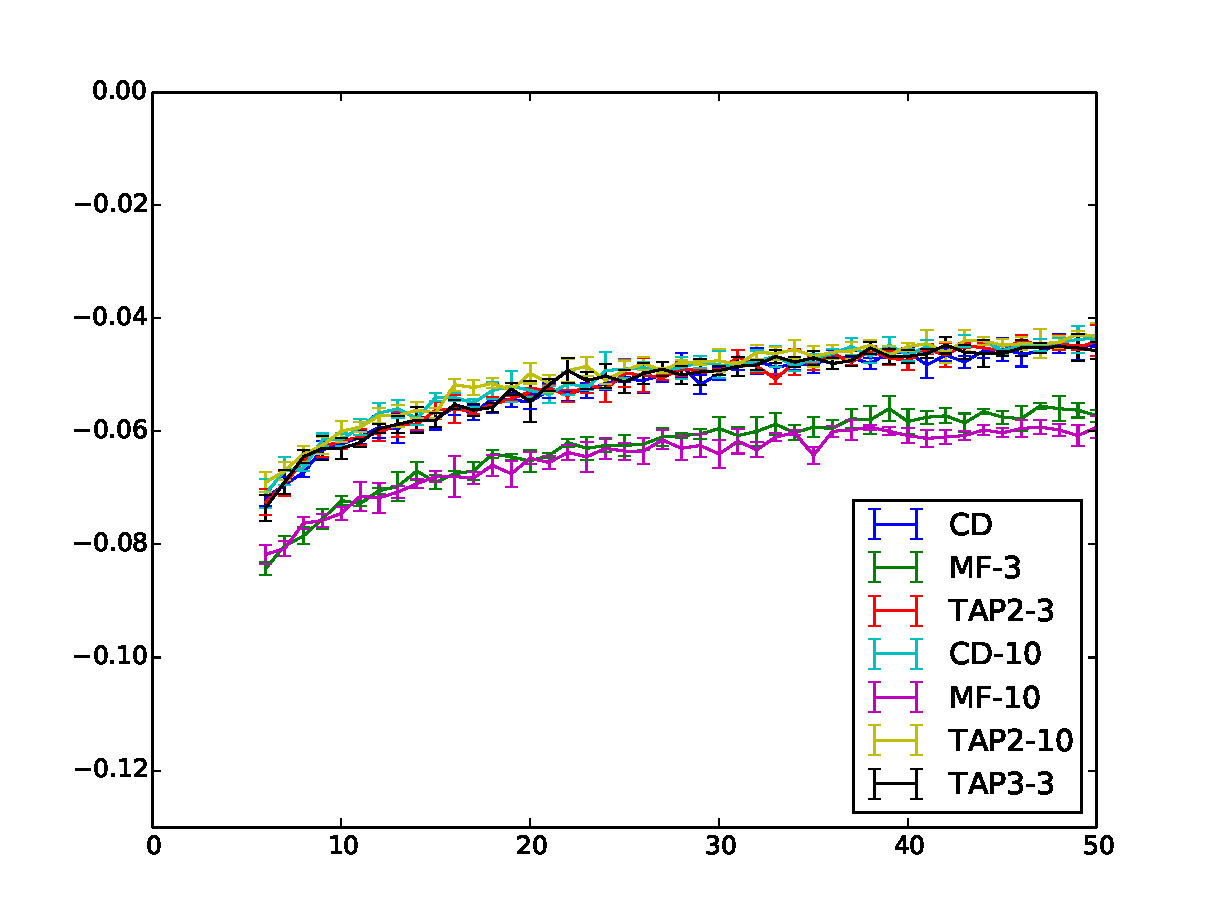
\includegraphics[width=\linewidth]{../../../Code/DRBM/scripts/validLL}
\endminipage 
\minipage{0.50\linewidth}  
 %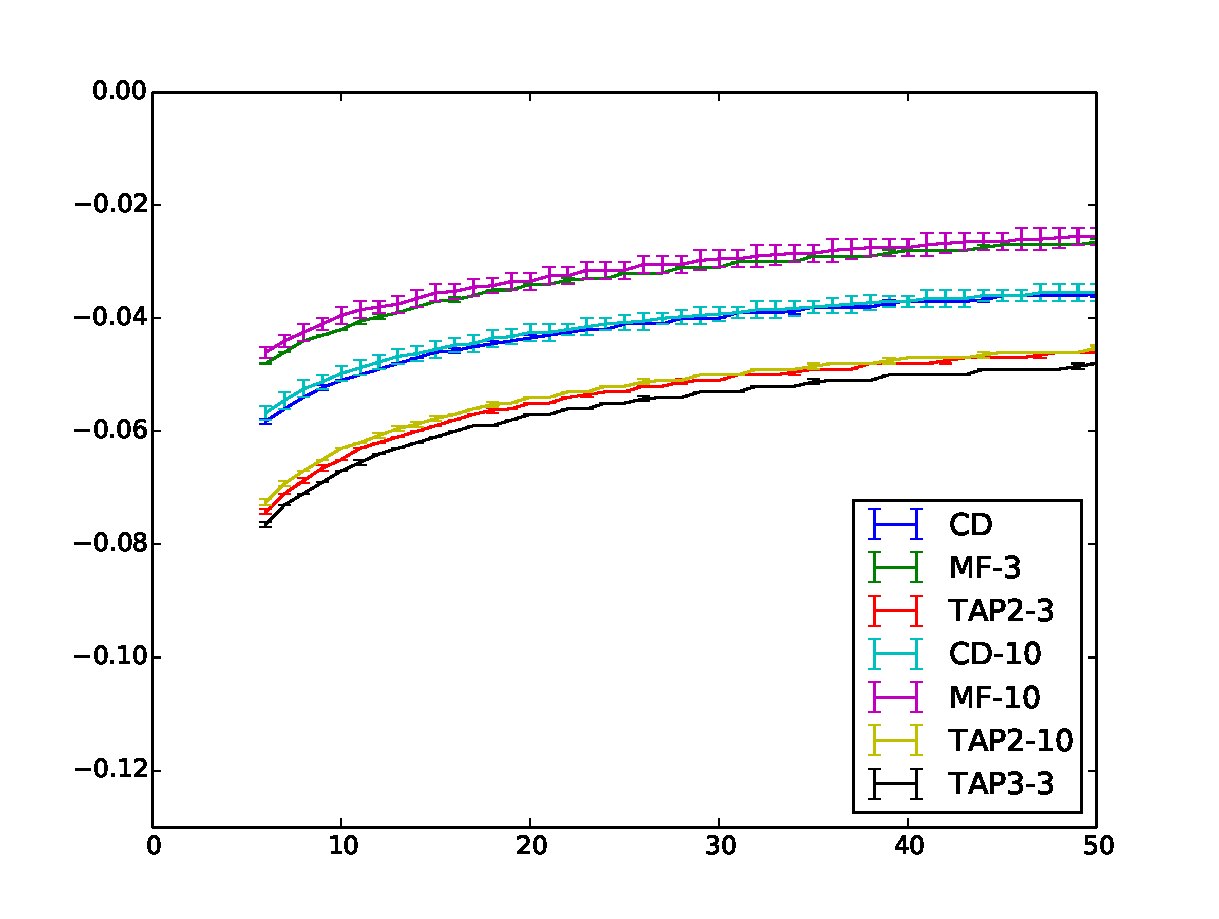
\includegraphics[width=\linewidth]{../../../Code/DRBM/scripts/validEMF}
\endminipage\hfill
  \caption[1]{Per-sample pseudo log-likelihood (left) and EMF log-likelihood (right) on the validation set of the MNIST data set divided by number of all units in the model ($1284$) across first training $50$ epochs for RBMs models trained stochastically and deterministically. Error bars shows the standard deviations of $10$ trained models using a particular version of training.}
   \label{fig:validLL}
\end{figure}
Secondly, results for the MF-10\footnote{The results for MF-3 weren't included as it was very similar to the MF-10} confirms the findings from the literature -- the naive mean field approach is not able to learn an effective model. Moreover, the results for the CD, TAP2 and TAP3 are very similar. There are not significant differences between models with $3$ or $10$ iterations of self-consistency relations which shows that the deterministic approach is not computationally expensive. 

As it was expected, the best results in terms of the EMF log-likelihood are achieved by EMF methods. However, the results for the CD models suggest that the EMF log-likelihood may be used as a reliable indicator of progress during training as those models weren't constructed to optimize over this objective \cite{gabrie2015training}.

Figure \ref{fig:PvalidLL} presents the results for persistent versions of models analysed above. There are not significant differences comparing to However, as it was expected the samples from the models trained using persistent chains are of much higher quality.
\begin{figure}[!htb]
\minipage{0.50\linewidth}
 \includegraphics[width=\linewidth]{../../../Code/DRBM/scripts/PvalidLL}
\endminipage 
\minipage{0.50\linewidth}  
 \includegraphics[width=\linewidth]{../../../Code/DRBM/scripts/PvalidEMF}
\endminipage\hfill
  \caption[1]{Per-sample pseudo log-likelihood (left) and EMF log-likelihood (right) for the same models trained using persistent Gibbs chains. Results of the naive method weren't included.}
   \label{fig:PvalidLL}
\end{figure}

Finally, in persistent and non-persistent versions of models the addition of the third order term from the EMF expansion \ref{eq:EMFexpansion} doesn't provide improvement over the TAP model. This might be partially explained by the fact that estimated weights are in general smaller than $1$ (in absolute value) which are then used at the order of $3$ in self-consistency equations and hence don't affect significantly estimations.

\subsection{Generated samples from the models}
The restricted Boltzmann machine can also be seen as a generative model that can creates new samples that will resemble the observed data provided that it approximates well the unknown distribution that generated the original, observed samples. Three models were trained with $500$ hidden units using persistent chains -- with the contrastive divergence algorithm, and two models using naive and extended mean field approach respectively. Figure \ref{fig:particles} shows samples generated from those models where between samples $1000$ chain steps were performed.
\begin{figure}[!htb]
\minipage{0.46\linewidth}%
 \includegraphics[width=\linewidth]{../../../Code/DRBM/backup/org/particles}
\endminipage 
\hfill
\minipage{0.46\linewidth}  
 \includegraphics[width=\linewidth]{../../../Code/DRBM/backup/mf/particles}
\endminipage
\vspace{2em}
  \minipage{0.46\linewidth}%
 \includegraphics[width=\linewidth]{../../../Code/DRBM/backup/pcd/particles}
\endminipage 
\hfill
\minipage{0.46\linewidth}  
 \includegraphics[width=\linewidth]{../../../Code/DRBM/backup/tap2/particlestap2}
\endminipage
  \caption[1]{Comparison of samples generated by $500$ hidden unit RBM trained using naive mean field approach (top right), extended mean field approximation up to the second-term order (bottom right) and with contrastive divergence (bottom left) to the original digits from the MNIST data (top left). All models were trained using persistent chains.}
  \label{fig:particles}
\end{figure}
The samples produced by the naive mean field methos provides the samples of the poorest quality that are often non-identifiable as one of $10$ digits. As we can see, the addition of the second-order term greatly improves also the generetive qualitative of the learned model. It might be argued that samples produced by the PCD and EMF models are of similar quality.

\chapter{Various experiments}

\section{Comparison of schedules of updates}
In the chapter $2$ different schedules of updates were analysed on toy models where the parameters of the model were known \emph{a priori} and no substantial discrepancies were observed in terms of the quality of approximation between asynchronous and parallel schedules. Taking into consideration the performance of the sequential updates on both toy models, this schedule wasn't considered in the evaluation on the real data set.

In the case of the MNIST data set, estimated magnetizations allow us to perform learning of unknown parameters. Thus, in this case we combine uncertainty related with both magnetizations and parameters -- this may lead to substantial differences in performance. Figure \ref{fig:updatesLL} shows the normalized estimates of log-likelihood of three models trained using the extended mean field approximation up to the first-order term (MF), up to the second-order term (TAP2) and up to the third-order term (TAP3), each trained with two nchedules of updates.

\begin{figure}[!htb]
\minipage{0.50\linewidth}%
\includegraphics[width=\linewidth]{../../../Code/DRBM/scripts/updatesMFLL.pdf}
\endminipage 
\minipage{0.50\linewidth}  
 \includegraphics[width=\linewidth]{../../../Code/DRBM/scripts/updatesMFEMF.pdf}
\endminipage\hfill

\minipage{0.50\linewidth}%
 \includegraphics[width=\linewidth]{../../../Code/DRBM/scripts/updatesTAP2LL.pdf}
\endminipage 
\minipage{0.50\linewidth}  
\includegraphics[width=\linewidth]{../../../Code/DRBM/scripts/updatesTAP2EMF.pdf}
\endminipage\hfill

\minipage{0.50\linewidth}%
\includegraphics[width=\linewidth]{../../../Code/DRBM/scripts/updatesTAP3LL.pdf}
\endminipage 
\minipage{0.50\linewidth}  
\includegraphics[width=\linewidth]{../../../Code/DRBM/scripts/updatesTAP3EMF.pdf}
\endminipage\hfill
  \caption[Estimates of log-likelihood with different updates]{Per-sample pseudo log-likelihood (left) and EMF log-likelihood (right) on the validation set of the MNIST data divided by number of all units in the model ($1284$) across first $50$ training epochs for RBMs models trained with different schedules and number of updates. Error bars show standard deviation of $10$ trained models using a particular version of training.}
  \label{fig:updatesLL}
\end{figure}

Surprisingly, only with the naive mean field approximation we can observe that the parallel schedule provides slightly better results in terms of the approximated log-likelihood. In general, there are no significant differences between two considered schedules even though the parallel form of updates doesn't reflect the way both layers of the RBM 'communicate' with each other. Moreover, it seems that small number of fixed point iterations doesn't deteriorate the performance. This suggests that asynchronous updates with only $3$ iterative updates of magnetizations yields consistently competitive results at the same time being the most computationally inexpensive form of schedule.

\subsection{Evaluation of EMF approximation}
The similiarity of the estimates of the log-likelihood using the pseudo log-likelihood method and with the extended mean field approach suggests that the high-temperature expansion method might be a computationally inexpensive metric of the partition function and the log-likelihood in general for RBMs. However, the pseudo log-likelihood is a very noisy approximation thus as a benchmark for comparison of the effectiveness of the EMF-based estimates I will use the annealed importance sampling (AIS) \cite{neal2001annealed} -- very popular method for computing the partition function. Naturally, this comparison assumes that the AIS estimate are close to the true value which in general might no be the case.
\section{Annealed Importance Sampling }
The AIS method is based on a very simple identity -- assume we have two distributions $p_A= \frac{1}{Z_A}p_A^*(\mathbf{x})$ and $p_B= \frac{1}{Z_B}p_B^*(\mathbf{x})$, where $p^*(\dot)$ denotes an unnormalized distribution and $Z_A, Z_B$ are partition functions of distribution $p_A$ and $B$ respectively. If the proposal distribution $p_A$ supports tractable sampling and tractable evaluation of both the unnormalized distribution $p_A^*(\mathbf{x})$ and the partition function $Z_A$, we can use the following relation:
\begin{align}
\begin{split}
Z_B & = \int p^*_B(\mathbf{x}) \text{d} \mathbf{x} \\ 
 &= \int \frac{p_A(\mathbf{x})}{p_A(\mathbf{x})} p^*_B(\mathbf{x}) \text{d} \mathbf{x}\\
 &=  Z_A \int \frac{ p^*_B(\mathbf{x}) }{ p^*_A(\mathbf{x}) }p_A(\mathbf{x})  \text{d} \mathbf{x} .
\end{split}
\end{align}
By sampling from the tractable distribution we can derive Monte Carlo estimator of the ratio between partition functions:
\begin{align}
\begin{split}
\frac{Z_B}{Z_A} \approx \frac{1}{N} \sum_{i=1}^N \frac{ p^*_B(\mathbf{x}^{(i)}) }{ p^*_A(\mathbf{x}^{(i)}) } = \hat{r}_{SIS}
\label{eq:ratioSIS}
\end{split}
\end{align}
where $\mathbf{x}^{(i)}$ comes from $p_A$.
Assuming that distribution $p_A$ is close to $p_B$, the estimator from  \ref{eq:ratioSIS} called simple importance sampling proves to work well \cite{minka2005divergence}. However, in high-dimensional spaces where $p_B$ is usually multimodal as it is considered in this thesis the variance of the estimator from \ref{eq:ratioSIS} might be very high. 

The idea presented above might be improved by following the classic approach from the probabilistic optimization i.e. simulated annealing. The idea is to introduce intermediate distributions that will allow to bridge the gap between two considered distributions $p_A$ and $p_B$ \cite{jarzynski1997nonequilibrium}, \cite{neal2001annealed}.

Consider a sequence of distributions $p_0, p_1, ..., p_M$ where $p_0 = p_A$ and $p_M = p_B$. If the intermediate distributions $p_{m}$ and $p_{m+1}$ are close enough, a simple estimator from \ref{eq:ratioSIS} can be used to estimate each ratio $\frac{Z_{m+1}}{Z_m}$. Using the identity: 
\begin{align}
\begin{split}
\frac{Z_M}{Z_0} = \frac{Z_1}{Z_0}\frac{Z_2}{Z_1}... \frac{Z_M}{Z_{M-1}}
\end{split}
\end{align}
those intermediate ratios are then combined to obtain the estimate of $\frac{Z_B}{Z_A}$. There is no need to compute the normalizing constants of any intermediate distributions. The intermediate distributions are chosen to suit a given problem domain. However, in most cases we are able to draw exact samples only from the first tractable distribution $p_A$. In order to sample from intermediate distribution we have be able to draw a sample $\mathbf{x}^{'}$ given $\mathbf{x}$ using Markov chain transition operator $T_m(\mathbf{x}^{'} |\mathbf{x}) $ that leaves $p_m(\mathbf{x})$ invariant, i.e.:
 \begin{align}
\begin{split}
\int T_m(\mathbf{x}^{'} |\mathbf{x}) p_m(\mathbf{x})\text{d}\mathbf{x} = p_m(\mathbf{x}^{'})
\end{split}
\end{align}
These transition operators represent the probability density of transitioning from state $\mathbf{x}$ to $\mathbf{x}^{'}$ \cite{salakhutdinov2008learning}. Having obtained the sequence of samples from the intermediate distributions we can obtain the improved estimator of the ratio between partition functions following the procedure:
\begin{algorithm}[!bthp]
\caption{Annealed importance sampling.}
\label{alg:vae}
\begin{algorithmic}
\State {Set $p_A$ and $p_B$ with appropriate parameters}
\For{$i \in \{1,..., N\} $} 
\State {sample $\mathbf{x}_{1}$ from $p_0 = p_A$} 
\State {sample $\mathbf{x}_{2}$ via $T_1(\mathbf{x}_{2} | \mathbf{x}_{1})$ }
\State ...
\State {sample $\mathbf{x}_{M}$ via $T_M(\mathbf{x}_{M} | \mathbf{x}_{M-1})$}
\State $r^{(i)}_{AIS} = \frac{ p^*_1(\mathbf{x}_1) }{ p^*_0(\mathbf{x}_1) }\frac{ p^*_2(\mathbf{x}_2) }{ p^*_1(\mathbf{x}_2) } ... \frac{ p^*_M(\mathbf{x}_M) }{ p^*_{M-1}
(\mathbf{x}_M) }$
\EndFor
  \State {$\hat{r}_{AIS} = \frac{1}{N} \sum_{i=1}^N \hat{r}^{(i)}_{AIS}$}
\end{algorithmic}
\end{algorithm}

It was proven that the variance of $\hat{r}_{AIS}$ will be proportional to $1 / MN$ assuming we used sufficiently large numbers of intermediate distributions $M$ \cite{neal2001annealed}. Moreover, the estimate of $Z_M / Z_0$ will be unbiased if each ratio is estimated using $N=1$ and a sample $\mathbf{x}^{m}$ is obtained using Markov chain starting at previous sample. This follows from the observation that the AIS procedure is an simple importance sampling defined on an extended state space $\mathcal{X} = (\mathbf{x}_1, \mathbf{x}_2, ..., \mathbf{x}_M)$.

The procedure described above can be adapted to the RBM case -- assume that we have estimated parameters $\mathbf{\theta}_B$ of the model that we want to evaluate. Following \cite{salakhutdinov2008quantitative} as a tractable starting distribution $p_A$ we can use "clamped" restricted Boltzmann machine where there is no hidden layer. The sequence of intermediate distribution is then defined as:
 \begin{align}
\begin{split}
p_m(\mathbf{v}) = \frac{1}{Z_m}p^*_m(\mathbf{v}) = \frac{1}{Z_m}\sum_\mathbf{h} \exp(-E_m(\mathbf{v, h}))
\end{split}
\end{align}
where $m = 0, ..., M$, $\mathbf{h} = \mathbf{h_B}$, and the energy function has the form:
 \begin{align}
\begin{split}
E_m(\mathbf{v,h}) = (1- \beta_m) E(\mathbf{v} ;\theta_A) + \beta_m E(\mathbf{v, h} ;\theta_B) 
\end{split}
\end{align}
where $\beta_m \in [0, 1]$ with $\beta_m = 0$ yielding $p_A$ and $\beta_m = 1$ giving $p_B$. By annealing slowly the "temperature" from infinity to zero we gradually moves from the state space of proposal distribution to the space defined by the untractable distribution.
% Following the approach from \ref{eq:TODOderivepropertiesofRBM} we can obtain transition operators for hidden and visible variables:
% \begin{align}
%\begin{split}
%p(h^A | \mathbf{v}) & = \sigma ((1 - \beta) NONE \\
%p(h^B) & =
%\end{split}
%\end{align}

\subsection{Comparison}
Two models were estimated based on the extended mean field approximation -- up to the second-order term (TAP2), and up to the third-order term (TAP3), to compare the quality of the approximation of the variational free energy.
Each model was re-estimated $10$ times using persistent chains with $10$ iterations of self-consistency relations with asynchronous updates. Taking into consideration the inherent variability of the AIS method, $10$ runs of AIS were performed to obtain an average estimate.  A sequence of $\beta$s is required to set the "tempo" of annealing -- following \cite{salakhutdinov2008learning} $1000$ $\beta_k$ were spaced uniformly from  $0 $ to  $0.5$, $4,000$ $\beta_k$ were spaced uniformly from $0.5$ to $0.9$, and $5,000$ $\beta_k$ were spaced uniformly from $0.9$ to $1.0$, with a total of 10,000 intermediate distributions. 

Firstly, both methods were compared on a small toy model where we can compute the true partition function explicitly -- an RBM with $15$ hidden units. Figure \ref{fig:AISTAP2small} presents the true value of the parition function along with its estimates from the TAP2 and TAP3 models and using the AIS method.

\begin{figure}[!htb]
\minipage{0.50\linewidth}%
 \includegraphics[width=\linewidth]{../../../Code/DRBM/scripts/smallAISTAP2}
\endminipage 
\minipage{0.50\linewidth}  
\includegraphics[width=\linewidth]{../../../Code/DRBM/scripts/smallAISTAP3}
\endminipage\hfill
  \caption[1]{Free energy estimates using two forms of extended mean field approximations and AIS estimates for $10$ trained models.}
  \label{fig:AISTAP2small}
\end{figure}

The results indicate that the AIS works rather well as an approximator of the true free energy. However, the EMF approximation tends to be biased and the addition of the third-order term improves the estimates only slightly. In both cases the approximation consistently overestimates the true value of $\mathcal{F}$ on average by about $5\%$. 

Having justified the usage of the AIS estimates as a benchmark, we can compare both methods on the RBM with $500$ hidden units. As a sanity check, the AIS was re-estimated in this case $100$ times as the results from \ref{salakhutdinov2008learning} show that the variance is then lower than $1\%$. Figure \ref{fig:AISTAP2small} presents the estimates of \ref{eq:freeEnergy} for the TAP2 and TAP3 models along with AIS estimates.

\begin{figure}[!htb]
\minipage{0.50\linewidth}%
 \includegraphics[width=\linewidth]{../../../Code/DRBM/scripts/AISTAP2}
\endminipage 
\minipage{0.50\linewidth}  
 \includegraphics[width=\linewidth]{../../../Code/DRBM/scripts/AISTAP3}
\endminipage\hfill
  \caption[1]{Free energy estimates using two forms of extended mean field approximations and AIS estimates for $10$ trained models.}
  \label{fig:AISTAP2}
\end{figure}

Firstly, as it was expected the learned models using two high-energy expansion yield very similar estimates of the free energy. Secondly, in both cases they give consistently biased upper bound approximation for the $\mathcal{F}$, assuming that the AIS method gives an accurate estimation of \ref{eq:freeEnergy}. As in the case of the toy model, the difference is about $5 \%$ in value on average. The mean squared error between the average AIS estimate and the TAP2 method was $505.747$ while for the the approximation including third-order the MSE was $534.193$. This suggests that even though the extended mean field approximation enable us to learn good generative models, the approximation of the free energy is very biased. However, the computational cost of estimation is about $10^{-5}$ smaller comparing to the AIS.

\section{Deep structures}
\subsection{Unsupervised pre-training of deep neural networks}
Recent major advances in tasks like speech recognition, vision recognition or machine translation were obtained thanks to effective training of deep neural structures. Deep learning methods allow to learn high-level features based on the composition of lower level characteristics. However, the objective function in general is highly non-convex and multi-modal over high-dimensional parameter space. This naturally leads to many challanges in training such deep structures.
 
The breakthrough that lead to effective training strategies for deep architectures came in 2006 with the CD algorithm for training deep belief networks (DBN) \cite{hinton2006reducing}. The deep structure might be formed by stacking single RBMs pre-trained using contrastive divergence approach. It was empirically shown that unsupervised pre-training guides the learning towards basins of attraction of minima that support better generalization from the training data set \ref{erhan2010does}. Thus, such pre-trained networks much better generalize and are more robust comparing to networks trained only in supervised fashion.

In the previous chapter it was shown that unsupervised learning using the extended mean-field approach can be used to learn a good quality generative model of the observed phenomena. Those results motivate learning deep structures using layer-wise greedily pre-training where instead of using CD for training RBMs we might consider fully deterministic approach. 
\subsection{Deep belief nets}
DBNs are generative graphical models with many hidden layers of hidden
causal variables which joint distribution has the following form:
\begin{align}
\begin{split}
p(\mathbf{x}, \mathbf{h}^1, \mathbf{h}^2,..., \mathbf{h}^l) = p(\mathbf{x}| \mathbf{h}^1)P(\mathbf{h}^1|\mathbf{h}^2)...
P(\mathbf{h}^{l-2}|\mathbf{h}^{l-1})P(\mathbf{h}^{l-1}|\mathbf{h}^{l}).
\end{split}
\end{align}
It was shown that adding an extra layers always improve a lower bound on the log-likelihood on the training data if the number of feature detectors per layer is sufficiently large and the weights are initialized correctly.  The guarantee that we improve the bound is no longer valid if the size of subsequent hidden layers is not large enough however it was empiracally proven that such approach still can learn an effective generative model. Figure \ref{fig:DBN} depicts the exemplary deep belief network. 

 \def\layersep{2.5cm}
\begin{figure}[!h]
\begin{center}
\begin{tikzpicture}[shorten >=1pt,->,draw=black!50, node distance=\layersep]
    \tikzstyle{every pin edge}=[<-,shorten <=1pt]
    \tikzstyle{neuron}=[circle,fill=blue!50,minimum size=17pt,inner sep=0pt]
    \tikzstyle{input neuron}=[neuron, fill=black!50];
    \tikzstyle{output neuron}=[neuron, fill=red!50];
    \tikzstyle{hidden neuron}=[neuron, fill=black!50];
     \tikzstyle{shidden neuron}=[neuron, fill=black!50];
          \tikzstyle{thidden neuron}=[neuron, fill=blue!50];
    \tikzstyle{annot} = [text width=4em, text centered]

    % Draw the input layer nodes
    \foreach \name / \y in {1,...,3}
    % This is the same as writing \foreach \name / \y in {1/1,2/2,3/3,4/4}       
     \node[input neuron, pin=left:Input \#\y] (I-\name) at (0,-\y) {};

    % Draw the hidden layer nodes
    \foreach \name / \y in {1,...,4}
        \path[yshift=0.5cm]
            node[hidden neuron] (H-\name) at (\layersep,-\y cm) {};

    % Draw the SECOND hidden layer nodes
    \foreach \name / \y in {1,...,4}
        \path[yshift=0.5cm]
            node[shidden neuron] (S-\name) at (2*\layersep,-\y cm) {};
            
            
    % Draw the THIRD hidden layer nodes
    \foreach \name / \y in {1,...,4}
        \path[yshift=0.5cm]
            node[thidden neuron] (T-\name) at (3*\layersep,-\y cm) {};

%    % Draw the output layer node
%    \node[output neuron,pin={[pin edge={->}]right:Output}, right of=S-3] (O) {};

    % Connect every node in the input layer with every node in the
    % hidden layer.
    \foreach \dest in {1,...,4}
    \foreach \source in {1,...,3}
            \path (H-\dest) edge  (I-\source);
            
% Connect every node in the hidden layer with every node in the
    % SECOND hidden layer.
            \foreach \dest in {1,...,4}
    \foreach \source in {1,...,4}
            \path (S-\dest) edge (H-\source) ;

% Connect every node in the hidden layer with every node in the
    % SECOND hidden layer.
    \foreach \source in {1,...,4}
        \foreach \dest in {1,...,4}
            \path (S-\source) edge (T-\dest);
      
      \foreach \dest in {1,...,4}
          \foreach \source in {1,...,4}
            \path (T-\dest) edge (S-\source) ;

    % Annotate the layers
    \node[annot,above of=H-1, node distance=1cm] (hl) {1th hidden layer};
    \node[annot,left of=hl] {Input layer};
        \node[annot,above of=S-1, node distance=1cm] (hl) {2nd hidden layer};
    \node[annot,above of=T-1, node distance=1cm] (hl) {3rd hidden layer};
\end{tikzpicture}
  \caption[Deep belief net]{An exemplary deep belief net with $3$ hidden layers where the last two layers form a single RBM.}
    \label{fig:DBN}
\end{center}
\end{figure}

Similarly to the case of the single RBM, DBN may be seen as a general approximator of any probability distribution on $\{0,1 \}^n$ and we can prove \cite{montufar2010refinements}
:
\begin{theorem} [Guido-Ay, 2010] Let $n = \frac{2^b}{2} + b$, $b \in \mathbb{N}$, $b \geqslant 1$. A DBN containing $\frac{2^n}{2(n-b)}$ hidden layers of size $n$ is a universal approximator of distributions on $\{0,1 \}^n$.
\end{theorem}

DBNs can be formed using a greedy layer-wise unsupervised training of stacked RBMs -- Algorithm \ref{alg:DBN} presents how the process folows.
\begin{algorithm}[!bthp]
\caption{Learning procedure for deep belief nets.}
\label{alg:DBN}
\begin{algorithmic}
\State {Train the first layer as an RBM, learning $P(\mathbf{x = h^{0}, h^1})$}
\For{$l \in \{2,..., L\} $} 
\State {Pass the mean activities $\mathbf{x}^l = P(\mathbf{h^{l}| \mathbf{h^{l-1}} })$ which become a representation of the input at the layer $l$.}
\State {Train the $l$-th layer treating it as an RBM with $\mathbf{x}^l$ as an input. }
\EndFor
\end{algorithmic}
\end{algorithm}
This simple and intuitive algorithm proved to be an effective way of pre-training deep structures that laid the foundations for the resurgence of deep neural networks. Originally, the building blocks are trained following constrastive divergence 
procedure.  However, the positive results obtained using the extended mean-field approximation suggests that we may follow Algorithm \ref{alg:DBN} with fully deterministic approach.

\subsection{Reconstruction analysis}
After pre-training multiple layers of feature detectors, the model can be ''unfolded'' to form an autoencoder structure where the decoder network uses transposed weigths of the encoder network. At this stage, such network might be considered as feed-forward deep neural architecture and might be used as a starting point for supervised fine-tuning with respect to any training criterion that depends on the learnt representation \ref{bengio2007greedy}.

To motivate the analysis of deep structures formed of stacked RBMs, I trained different three models that compress the information in the data to $25$ dimensional manifold -- using principal component analysis with first $25$ dimension with the highest variance, Check, a single RBMs with $25$ hidden units and a deep belief net that consists of three hiddent layers of sizes $500$, $250$ and $25$. Both models were trained using an extended mean field approach up to the second-order term with persistent chains.

\begin{figure}[!htb]
\includegraphics[width=\linewidth]{../../../Code/DRBM/drbm/reconstructions2}
  \caption[Reconstruction of digits with basic models]{Reconstructions of MNIST digits (top row) generated by PCA-25 (second row),  single RBM with $25$ hiddent units (third row) and deep belief net (bottom row).}
  \label{fig:pca}
\end{figure}
As we can see, the linear transformation to the small dimensional space creates very noisy encoding system. The reconstructions show that the numbers lie very closely on the space from which we decode. The reconstructions provided by the single RBM substanitally improves the quality of the reconstructions and it can be infer that the learned manifold better differentiate between the digits. However, although the background is properly delimited from the numbers, digits are still very blurry. It might be argued that the deep structure creates the most sharply-outlined numbers. From this we might infer that deep belief net is able to creates more coarser and coarser features that in the process of the encoding are able to generate clear-cut digits as the learned meanifold in the smallest layer is properly partitioned.

Similarly to the case of the shallow structures, we might compare the effectiveness of the EMF approach to the CD learning in the case of the greedily layer-wise training of DBN. Figure \ref{fig:drbm} presents the reconstructions of randomly chosen samples from the validation data set produced by deep autoencoders trained with four different methods of pre-training DBNs. The autoencoder consists of three hidden layers of sizes $500$, $250$ and $25$ accordingly. Extended mean field approximation was considered up to the first-order (MF), second-order (TAP2) and third-order (TAP3) terms. One model was also trained using CD procedure. At each layer $50$ updates through the entire data sets were performed using $10$ iterations of asynchronous updates. In each case magnetization or Gibbs chains were persistent.

\begin{figure}[!htb]
\includegraphics[width=\linewidth]{../../../Code/DRBM/drbm/reconstructions}
  \caption[Reconstructions of digits with deep structures]{Reconstructions of MNIST digits (top row) generated by four different deep belief nets trained using naive mean field approach (second row), EMF up to the second-order term (third row), EMF up to the third-order term (fourth row) and with PCD (bottom row).}
\label{fig:drbm}
\end{figure}
  
%Figure \ref{fig:drbm} presents the reconstructions of MNIST digits as well as a the original numbers. 
By the visual inspection, it might be argued that the reconstruction created by TAP2, TAP3 and PCD are of similar quality and they are more identifiable than those produced by the MF. 
It can be observed how the autoencoder learnt by EMF or PCD recovers a a smoothed version of the original digit -- an "average" representative of a given number. Surprisingly, the addition of the third-order term leads somewhat to deterioration of the quality in reconstructions which can be observed especially in the case of the first ($2$) and sixth ($5$) number. 
The average squared errors on training and validation data sets (Figure \ref{fig:mse}) confirms the visual assessment of reconstructions. The mean field approximation obtains the highest score while TAP2 and TAP3's scores are slightly higher than with training DBN using PCD approach. 

\begin{figure}[!htb]
\begin{center}
\includegraphics[width=.5\linewidth]{../../../Code/DRBM/drbm/mseRecon}
\end{center}
  \caption[1]{MSE of reconstructions for four different models on training and validation sets.}
\label{fig:mse}
\end{figure}

Those results confirms the observations from the previous chapter and shows that additional higher-order approximations substantially improves the quality of learned magnetizations which in turns helps learning a better generative model.

%\subsection{Semi RBM}
%SEE IF IT IS WORTH IT.
%\subsubsection{Exploiting the SRBM structure}
%Clamped free energy can be written in the form:
%\begin{align}
%\begin{split}
%\mathcal{F}^c(\mathbf{v}) = & \sum_\mathbf{h} e^{-E(\mathbf{v}, \mathbf{h})} = e^{\mathbf{b}'\mathbf{v}}\sum_{h_1}...\sum_{h_m}e^{-E(\mathbf{v}, \mathbf{h})} \\
%=&  e^{\mathbf{b}'\mathbf{v}} \sum_{h_1} e^{h_1 (c_1 + W_{1\bullet}\mathbf{v})}... \sum_{h_m} e^{h_m (c_m + W_{m\bullet}\mathbf{v})} \\
%= & e^{\mathbf{b}'\mathbf{v}} \prod_{j=1}^{m} \left( 1 + e^{c_i + W_{i\bullet}\mathbf{v}} \right)
%\label{eq:freeEnergy}
%\end{split}
%\end{align}

\chapter*{Conclusions}
\addcontentsline{toc}{chapter}{Conclusions}
Variational approximation to the untractable free energy using high-temperature perturbation expansion brings significant improvements over the naive mean field approach applied to bipartite structures, specifically to the restricted Boltzmann machine. Even though the expansion is performed around the point where all spins are independent, the radius of convergence is large enough to obtain robust results for smaller temperatures. By adding higher-order terms from a systematic expansion, we are able to model dependence between variables possibly at arbitrarily order.

Experiments on toy models confirmed first promising results on the real data set shown by Gabri{\'e} et al. \cite{gabrie2015training}. Additional terms responsible for couplings and triplets of units greatly improve training efficiency and performance over the naive mean field approach in the case of the RBM structure. Those improvements can be observed even in the case of a very small model. Remarkably, for the grid model the extended approach performs worse than the naive one which might be explained by the fact that the averaging implicitly assumed in the latter case is consistent with the structure of the grid. Moreover, I analysed three different schedules of updates of magnetizations -- the results suggest that the EMF method is rather robust to the different schemes as long as the updates are performed layer-wise. Interestingly, in that case parallel updates yields similar results as an asynchronous scheme.

The quality of estimates and learned generative models is retained in the case of the real data set. The extended mean field approximation provides performance comparable and sometimes superior to contrastive divergence procedure -- the most widely used procedure for pre-training RBMs and DBNs. The experiments confirmed the previous observations that even with only $3$ iterations of magnetizations we are able to train generative models that produce samples of good quality. This shows that the EMF method might be used when fast deterministic training is desired.

The experiments performed on the real data set yields results that are in accordance to the ones obtained on toy models. No differences were observed between parallel and asynchronous updates which suggests that this method might be applied to more complicated graphs' structures. Unsatisfactorily the comparison with annealed importance sampling shows that the EMF approximation of the partition function is strongly biased even with a small number of hidden units. However, the computational cost is significantly lower and  this method might be used if we need a ballpark figure of the value of the partition function during training. Moreover, the AIS procedure needs to be adapted to specific structure of the model while the EMF approximation can be used with any energy based model defined over binary variables.

The natural generalization to training deep structures was suggested where deep belief nets are pre-trained using greedy layer-wise deterministic procedure based on the EMF approximation. The hierarchical structure enables to process information through multiple stages of transformation which results in better reconstructions than shallow structures. Results also suggest that this procedure allows to initialize weights effectively for supervised training later on. As it was the case for the single RBM, the deterministic algorithm achieves comparable performance to stochastic procedure based on the contrastive divergence algorithm.

OPPER  mannfredintro to general case.TODO possibsdsly to extend the approach to arbitrary order.

The code needed to replicate all results is available at \url{https://github.com/budzianowski/DRBM}. 



% ********************************** Back Matter *******************************
% Backmatter should be commented out, if you are using appendices after References
%\backmatter

% ********************************** Bibliography ******************************
\begin{spacing}{0.9}

% To use the conventional natbib style referencing
% Bibliography style previews: http://nodonn.tipido.net/bibstyle.php
% Reference styles: http://sites.stat.psu.edu/~surajit/present/bib.htm

\bibliographystyle{apalike}
%\bibliographystyle{unsrt} % Use for unsorted references  
%\bibliographystyle{plainnat} % use this to have URLs listed in References
\cleardoublepage
\bibliography{References/references} % Path to your References.bib file

% If you would like to use BibLaTeX for your references, pass `custombib' as
% an option in the document class. The location of 'reference.bib' should be
% specified in the preamble.tex file in the custombib section.
% Comment out the lines related to natbib above and uncomment the following line.

%\printbibliography[heading=bibintoc, title={References}]

\end{spacing}

% ********************************** Appendices ********************************

\begin{appendices} % Using appendices environment for more functunality
% ******************************* Thesis Appendix A ****************************
\chapter{EMF derivation} 

Following \cite{georges1991expand} lets define
energy as:
\begin{align}
\begin{split}
E = -\sum_{ij} w_{ij}s_i s_j - \sum_i \theta_i s_i
\end{split}
\end{align}
and introduce the following operator:
\begin{align}
\begin{split}
U \equiv E - \mathbb{E}(E) - \sum_i \frac{\partial \lambda_i (\beta)}{\partial \beta} (s_i - m_i)
\label{eq:Uoperator}
\end{split}
\end{align}
which poses useful property -- $\mathbb{E}(U) = 0$. For any other operator $O$ we then have:
\begin{align}
\begin{split}
 \frac{\partial \mathbb{E}(O)}{\partial \beta}  =   \mathbb{E} \left(\frac{\partial O}{\partial \beta} \right) - \mathbb{E}(OU).
 \label{eq:obeta}
\end{split}
\end{align}
Now, the first derivative from the Taylor expansion is:
\begin{align*}
\begin{split}
\frac{\partial (\beta F)}{\partial \beta} = &
\dfrac{\sum_{\mathbf{s}} \exp \left( \beta \sum_{(ij)} w_{ij} s_i s_j +  \beta \sum_i \theta_i s_i+ \sum_i \lambda_i (\beta) (s_i - m_i) \right) \left(\sum_{(ij)} w_{ij} s_i s_j +  \sum_i \theta_i s_i + \sum_i \frac{\partial \lambda_i(\beta)}{\partial \beta} (s_i - m_i) \right) }
{\sum_{\mathbf{s}} \exp \left( \beta \sum_{(ij)} w_{ij} s_i s_j + \sum_i \theta_i s_i + \sum_i \lambda_i (\beta) (s_i - m_i) \right)} \\
 = & \sum_{(ij)} w_{ij} \mathbb{E}(  s_i s_j) +  \sum_i a_i  \mathbb{E}( s_i) + \frac{\partial \lambda_i(\beta)}{\partial \beta} \sum_i \mathbb{E}(
 s_i - m_i ).
\end{split}
\end{align*}
In the case of $\beta = 0$ we have:
$$ \left. \frac{\partial (\beta F)}{\partial \beta}\right|_{\beta = 0} = \sum_{(ij)} w_{ij} m_i m_j +  \sum_i \theta_i m_i .$$
Using \ref{eq:obeta} we obtain:
\begin{align}
\begin{split}
\frac{\partial m_i}{\partial \beta} = 0 = \frac{\partial \mathbb{E}(s_i)}{\partial \beta}  =   \mathbb{E} \left(\frac{\partial s_i}{\partial \beta} \right) - \mathbb{E}(s_iU) =- \mathbb{E}(s_iU)  =- \mathbb{E}(U(s_i - m_i)).
\end{split}
\end{align}
The first derivative of the operator $U$ has the form:
\begin{align}
\begin{split}
\frac{\partial U}{\partial \beta}  =  ~&\frac{\partial E}{\partial \beta} - \frac{\partial \mathbb{E}(E)}{\partial \beta} - \sum_i \frac{\partial^2 \lambda_i (\beta)}{\partial \beta^2} (s_i - m_i)\\
= ~& \mathbb{E}(U^2) - \sum_i \frac{\partial^2 \lambda_i (\beta)}{\partial \beta^2} (s_i - m_i)
\end{split}
\end{align}
and the second derivative is:
\begin{align}
\begin{split}
\frac{\partial^2 U}{\partial \beta^2}  =  ~& 2 \mathbb{E}\left(\frac{\partial U}{\partial \beta}U  \right) - \mathbb{E}(U^3) - \sum_i \frac{\partial^3 \lambda_i (\beta)}{\partial \beta^3} (s_i - m_i) \\
= ~& - \mathbb{E}(U^3) - \sum_i \frac{\partial^3 \lambda_i (\beta)}{\partial \beta^3} (s_i - m_i)
\end{split}
\end{align}
The expansion of free energy using formulas derived above can now be reformulated in terms of the operator $U$:
\begin{align}
\begin{split}
 \frac{\partial (\beta F)}{\partial \beta} = \mathbb{E}(E) - \sum_i \frac{\partial\lambda_i (\beta)}{\partial \beta}\mathbb{E}(s_i - m_i) = \mathbb{E}(E) 
\end{split}
\label{eq:naive}
\end{align}
and the higher orders:
\begin{align}
\begin{split}
 \frac{\partial^2 (\beta F)}{\partial \beta^2} = &~ \mathbb{E}\left( \frac{\partial E}{\partial \beta} \right) - \mathbb{E}(EU) = - \mathbb{E}(U^2),\\
 \frac{\partial^3 (\beta F)}{\partial \beta^3}= &~ - 2\mathbb{E}\left( U \frac{\partial U}{\partial \beta} \right) + \mathbb{E}(U^3)  = \mathbb{E}(U^3).
  \label{eq:higherOrders}
\end{split}
\end{align}
Taylor expansion was considered around point $\beta =0$. Using derivations from \ref{eq:naive} we obtain again a 'naive' term:
\begin{align}
\begin{split}
\left. \frac{\partial (\beta F)}{\partial \beta} \right|_{\beta =0} = \mathbb{E} _{\beta = 0}(E) = - \sum_{(ij)} w_{ij} m_i m_j - \sum_i \theta_i m_i = - \frac{1}{2} \sum_i \sum_j w_{ij}m_i m_j - \sum_i \theta_i m_i.
\end{split}
\end{align}
Consider now:
\begin{align}
\begin{split}
\left.\frac{\partial (\beta F)}{\partial m_i \partial \beta}\right|_{\beta = 0} = 
- \sum_{j \neq i} w_{ij} m_j - \theta_i.
\end{split}
\end{align}
On the other hand:
\begin{align}
\begin{split}
\left. \frac{\partial (\beta F)}{\partial m_i \partial \beta}\right|_{\beta = 0} = \left. \frac{\partial (\beta F)}{\partial \beta \partial m_i }\right|_{\beta = 0} = \frac{\partial}{\partial \beta} \mathbb{E} (\lambda_i(\beta)) =  \left. \frac{\partial \lambda_i (\beta)}{\partial \beta}\right|_{\beta =0}
 \label{eq:maxwell}
 \end{split}
\end{align}
Substituting  \ref{eq:maxwell} into \ref{eq:Uoperator} gives us:
\begin{align}
\begin{split}
U_{\beta = 0} = & -\sum_{(ij)} w_{ij}s_is_j -\sum_i \theta_i s_i + \frac{1}{2} \sum_i \sum_j w_{ij} m_i m_j + \sum_i \theta_i m_i + \sum_i \left(\sum_{j \neq i} w_{ij} m_j  + \theta_i \right)(s_i - m_i ) \\
= & -\sum_{(ij)} w_{ij}s_i s_j - \frac{1}{2}\sum_{(ij)} w_{ij} m_i m_j + \sum_i \sum_{j \neq i} w_{ij} s_i m_j \\
= & - \sum_{(ij)} w_{ij} (s_i - m_i)(s_j- m_j) = - \sum_l w_l y_l
 \end{split}
\end{align}
where $w_l = w_{ij}$ and $y_l = (s_i -m_i)(s_j-m_j)$ stands for the 'link' operator which poses useful properties:
\begin{align}
\begin{split}
\mathbb{E}(y_l)_{\beta =0} = & ~\mathbb{E}(s_i s_j) -m_j\mathbb{E}(s_i) - m_i\mathbb{E}(s_j) + m_i m_j = 0 \\
\mathbb{E}(y_l(s_i-m_i))_{\beta =0} = & ~ m_j - m_j -m_i^2m_j + m_i^2m_j \\
 & ~ - m_i^2m_j + m_i^2m_j + m_i^2m_j - m_i^2m_j \\
 = &~ 0.
 \end{split}
\end{align}
Finally, if $k \neq l$ then:
$$\mathbb{E}(y_k y_l)= \mathbb{E}(y_k)\mathbb{E}(y_l)=0$$
while for $k = l$ we have:
\begin{align}
\begin{split}
\mathbb{E}((s_i-m_1)^2(s_j-m_j)^2)= & ~m_im_j - 2m_im_j^2 +m_im_j^2 - 2m_i^2m_j + 4m_1^2m_j^2\\
& - 2m_i^2m_j^2 + m_i^2m_j -2m_i^2m_j^2 + m_i^2m_j^2 \\
= & ~ (m_i -m_i^2)(m_j-m_j^2).
\label{eq:Yoperator}
 \end{split}
\end{align}
Using properties from $y_l$ in equations \ref{eq:higherOrders} we can derive:
\begin{align*}
\begin{split}
\left. \frac{\partial^2 (\beta F)}{\partial \beta^2}\right|_{\beta = 0} = & -\mathbb{E}(U^2)_{\beta =0}\\
= & - \sum_{l_i l_2} w_{l_i}w_{l_2} \mathbb{E}_{\beta = 0} (y_{l_1}y_{l_2} ) \\
= & - \sum_{(i,j)} w_{ij}^2 (m_i-m_i^2)(m_j-m_j^2)
\end{split}
\end{align*}
which yields the TAP-Onsager term. 
%ing approach from \ref{eq:maxwell} we have:
%\begin{align*}
%\begin{split}
%\left.\frac{\partial^2 \lambda_i (\beta)}{\partial \beta^2}\right|_{\beta =0} = \left.\frac{\partial^3 (\beta G)}{\partial m_i \partial \beta^2}\right|_{\beta = 0} = 2m_i \sum_{j \neq i} w_{ij}^2(1-m_j^2)
%\end{split}
%\end{align*}
To obtain the next term in the Taylor expansion we need to compute $\mathbb{E}(y_{l_1} y_{l_2} y_{l_3})$ term and by definition the structure of the RBM model doesn't admit triangles in its corresponding factor graphs. Thus, we need to consider only the case when $l_1 = l_2 = l_3$:
\begin{align}
\begin{split}
\mathbb{E}((s_i-m_1)^3(s_j-m_j)^3)= & ~m_i m_j -3m_i m_j^2 +2 m_i m_j^2 + 2m_im_j^3 -3 m_i^2 m_j 
 + 2 m_i^3 m_j \\
 & + 9 m_i^2m_j^2 - 6m_i^3 m_j^2 - 6 m_i^2 m_j^3 + 4m_i^3m_j^3 
 \\
  = &~ 4(m_i - m_i^2)(\frac{1}{2} - m_i)(m_j - m_j^2)(\frac{1}{2} - m_j)
 \end{split}
\end{align}
and the third-order term in the case of the RBM structure:
\begin{align*}
\begin{split}
\left. \frac{\partial^3 (\beta F)}{\partial \beta^3}\right|_{\beta = 0} = \frac{2\beta^3}{3} \sum_{(ij)} w_{ij}^3 (m_i - m_i^2)(\frac{1}{2} - m_i)(m_j - m_j^2)(\frac{1}{2} - m_j).
\end{split}
\end{align*}



\end{appendices}

% *************************************** Index ********************************
\printthesisindex % If index is present

\end{document}
